\documentclass{article}
%build with recipe latexmk
\usepackage[utf8]{inputenc}
\usepackage[T1]{fontenc}
\usepackage{textcomp}
\usepackage{fancyhdr}
\pagestyle{fancy}
%\addtolength{\headwidth}{\marginparwidth}
%\addtolength{\headwidth}{\marginparsep}
%\addtolength{\headwidth}{\marginparsep}
\usepackage{tcolorbox}
\tcbuselibrary{theorems}
\usepackage{babel}
\usepackage{enumerate}
\usepackage{amsmath, amssymb, amsthm}
%\usepackage{a4wide}
\usepackage{float}
\usepackage{tikz-cd}
\usepackage{tikz}
\usepackage{graphicx}
\usepackage{caption}
\usepackage{wrapfig}
\graphicspath{ {./images/} }
\usepackage{setspace}
\setstretch{1.1}
\usepackage{color}
\usepackage{hyperref}
\hypersetup{
    colorlinks=true, %set true if you want colored links
    linktoc=all,     %set to all if you want both sections and subsections linked
    linkcolor=black,  %choose some color if you want links to stand out
}

\theoremstyle{definition}
\newtheorem{theorem}{Theorem}[section]
\newtheorem{lemma}[theorem]{Lemma}
\newtheorem{cor}[theorem]{Corollary}
\newtheorem{prop}[theorem]{Proposition}
\newtheorem{example}{Example}[section]
\newtheorem{defn}{Definition}[section]

\title{ Part II - Galois Theory
    \\ \large
Lectured by Prof. A. J. Scholl
}
\author{Artur Avameri}
\date{Michaelmas 2022}

% figure support
\usepackage{import}
\usepackage{xifthen}
\pdfminorversion=7
\usepackage{pdfpages}
\usepackage{transparent}
\newcommand{\incfig}[1]{%
    \def\svgwidth{\columnwidth}
    \import{./figures/}{#1.pdf_tex}
}

\pdfsuppresswarningpagegroup=1

\setcounter{section}{-1}
\begin{document}
\maketitle
\tableofcontents
\newpage

\section{Introduction}

\marginpar{06 Oct 2022, Lecture 1}


Galois Theory begins with polynomial equations and trying to solve them. Galois discovered certain \textbf{symmetries} of equations, which led to symmetries of fields (Steinitz, Artin).

\vspace{1mm}


Babylonians were able to solve the quadratic equation $X^2 + bX + c$ thousands of years ago, and so can we - write it as $(X + b/2)^2 + c - b^2/4$, which leads to the quadratic formula, or use Vieta's formulas to get $x_1x_2 = c, x_1 + x_2 = -b$, from which we can solve for $x_1$ by doing $x_1 = \frac{1}{2} \left( (x_1 + x_2) + (x_1 - x_2) \right)$ and $(x_1 - x_2)^2 = (x_1 + x_2)^2 - 4x_1x_2$.

\vspace{1mm}


A lot later people figured out how to solve the cubic equation, $X^3 + aX^2 +bX + c$. We get $x_1 + x_2 + x_3 = -a, x_1x_2 + x_2x_3 + x_3x_1 = b, x_1x_2x_3 = -c$. If we replace $X \mapsto X- a/3$, we end up with a cubic equation without a quadratic term. Now \[
x_1 = \frac{1}{3}\left[(x_1+x_2+x_3) + (x_1 + \omega x_2 + \omega^2 x_3) + (x_1 + \omega^2 x_2 + \omega x_3) \right]
\] for $\omega = e^{2\pi i/3}$ a cube root of unity. Let $u = (x_1 + \omega x_2 + \omega^2 x_3), v = (x_1 + \omega^2 x_2 + \omega x_3)$.

If we cyclically permute $x_1,x_2,x_3$, we find $u \mapsto \omega u \mapsto \omega^2 u$ and $v \mapsto \omega v \mapsto \omega^2 v$, so $u^3$ and $v^3$ are invariant under cyclic permutations of the roots. Hence $u^3+v^3$ and $u^3v^3$ are invariant under permutations of the roots, so (as we prove in the next lecture) we can express them in terms of the coefficients of the polynomial.

In fact, they're given by $u^3 + v^3 = -27c, u^3v^3 = -27b^2$, hence $u^3,v^3$ are roots of $Y^2 + 27cY - 27b^2$, from which we can find $u,v$ and hence $x_1$. This is \textbf{Cardano's formula}.

\vspace{1mm}

If we proceed similarly for quartics, we end up with a cubic equation which we can solve as above. Unfortunately, this doesn't work for quintics. The reason for this lies in group theory.

\newpage

\section{Polynomials}

In this course, all rings will be commutative, with a one, and nonzero. For a ring $R$, $R[X]$ is the ring of polynomials over $R$, i.e. just the formal expressions $\sum_{i=0}^{n} a_i X^i$ for $a_i \in R$.

A polynomial $f \in R[X]$ determines a \textbf{function} $R \to R$. However, the polynomial $r \mapsto f(r)$ isn't in general determined by the function. For example, if $R = \mathbb{Z}/p\mathbb{Z}$ for $p$ a prime, then $\forall a \in R, a^p = a$, so the polynomials $X^p$ and $X$ represent the same function, while being different polynomials.

In the case where $R = K$ is a field, we know $K[X]$ is a Euclidean domain, so it has a division algorithm: if $f,g \in K[X]$ and $g$ is nonzero, then there exist unique $q,r$ such that $f = gq + r$ and $\text{deg}(r) < \text{deg}(g)$ (note that $\text{deg}(0) = - \infty$). If $g = X-a$ is linear, then we get $f =(X-a)q + f(a)$, the \textbf{remainder theorem}.

$K[X]$ is also a PID and UFD, so every polynomial is a product of irreducible polynomials, and there are GCDs, which we can compute using Euclid's algorithm.

\begin{prop}
    If $K$ is a field and $f \in K[x]$ is nonzero, then $f$ has at most $\text{deg}(f)$ roots in $K$.\footnote{Note that this is not true if $K$ is a ring.}
\end{prop}
\begin{proof}
    If $f$ has no roots, we're done. Otherwise, let $f(a) = 0$ and write ${f = (X-a)g}$ with $\text{deg}(g) = \text{deg}(f) - 1$. But if $b$ is a root of $f$, then ${f(b) = 0} \implies b=a$ or $g(b)=0$, so $f$ has at most $(1 + \text{number of roots of }g)$ roots and the claim follows by induction.
\end{proof}

\section{Symmetric polynomials}

Let $R$ be a ring and consider $R[X_1, \ldots, X_n]$ for some $n\ge 1$.
\begin{defn}
    A polynomial $f \in R[X_1,\ldots, X_n]$ is \textbf{symmetric} if for every permutation $\sigma \in S_n$, $f(X_{\sigma(1)}, \ldots, X_{\sigma(n)}) = f$.
\end{defn}

The set of symmetric polynomials is a subring of $R[X_1,\ldots,X_n]$.

\begin{example}
    $X_1 + \ldots + X_n$, or more generally, $P_k = \sum_{i=1}^{n} X_i^k$ are symmetric polynomials.
\end{example}

Alternative definition:
\begin{defn}
    If $f \in R[X_1,\ldots,X_n]$, define $f \sigma = f(X_{\sigma(1)}, \ldots, X_{\sigma(n)})$. This is a (right) action on the group $S_n$. We say $f$ is \textbf{symmetric}  if $f \sigma = f ~\forall \sigma \in S_n$.
\end{defn}

The \textbf{elementary symmetric polynomials} are \[
    s_r(X_1, \ldots, X_n) = \sum_{i_1 < \ldots < i_r}^{} X_{i_1}\ldots X_{i_r}.
\]
\begin{example}
    For $n=3$, $s_1 = X_1 + X_2 + X_3$, $s_2 = X_1X_2 + X_1X_3 + X_2X_3$, $s_3 = X_1X_2X_3$.
\end{example}

\begin{theorem}%theorem 2.1 in lectures
    \begin{enumerate}[(i)]
        \item Every symmetric polynomial over $R$ can be expressed as a polynomial in $\{s_r ~|~ 1\le r\le n\}$ with coefficients in $R$.
        \item There are no non-trivial relations between $s_1, \ldots, s_n$ - they're independent.
    \end{enumerate}
\end{theorem}

\marginpar{08 Oct 2022, Lecture 2}

\textbf{Remarks.} \begin{enumerate}[(a)]
    \item Consider the homomorphism $$\theta: R[Y_1,\ldots,Y_n] \to R[X_1,\ldots,X_n]$$ by ${\theta(Y_r) = S_r}$ (and identity on $R$). Then (i) says that the image of $\theta$ is the set of symmetric polynomials, and (ii) says that $\theta$ is injective.
    \item An equivalent definition of the $\{s_r\}$ is $$\prod_{i=1}^{n} (T+x_i) = T_n + s_1 T^{n-1} + \ldots + s_{n-1}T + s_n.$$
    \item If we need to specify the number of variables, we write $s_{r,n}$ instead of $s_r$.
\end{enumerate}

\begin{proof}[Proof of Theorem 2.1.]
    Terminology:
    \begin{itemize}
        \item A \textbf{monomial} is some $X_{I} = X_1^{i_1}\ldots X_n^{i_n}$ for some $I \in \mathbb{Z}_{\ge 0}^n$.
        \item Its \textbf{(total) degree} is $\sum_{}^{} i_\alpha$.
        \item A \textbf{term} $\beta$ is some $c X_I, 0 \neq c \in R$, so a polynomial is uniquely a sum of terms.
        \item The total degree of $f$ is the maximal degree of any of the terms.
    \end{itemize}

    Define a lexicographical ordering on monomials $X_I$ as follows: $X_I > X_J$ if either $i_1 > j_1$ or for some $1 \le r < n$, $i_1=j_1,\ldots, i_r = j_r$ and $i_{r+1} > j_{r+1}$. This is a \textbf{total ordering}: for each pair $I \neq J$, exactly one of $X_I > X_J$ or $X_J > X_i$ holds.

    Existence: Let $d$ be the total degree of some symmetric polynomial $f$ and let $X_I$ be the lexicographically largest monomial in $f$ with coefficient $c \in R$. As $f$ is symmetric, we must have $i_1\ge i_2 \ge \ldots \ge i_n$ (if not, say $i_r < i_{r+1}$, then exchanging $X_r$ and $X_{r+1}$ gives a monomial occuring in $f$ which is bigger than $X_I$).
    So $$X_I = X_1^{i_1-i_2}(X_1X_2)^{i_2-i_3}\ldots(X_1\ldots X_n)^{i_n}.$$
    Consider $g = s_1^{i_1-i_2}s_2^{i_2-i_3}\ldots s_{n-1}^{i_{n-1}-i_n}s_n^{i_n}$. The leading monomial (i.e. largest in lexicographical order) of $g$ is $X_I$, and $g$ is symmetric, so $f-cg$ is also symmetric, of total degree $\le d$, and its leading term is smaller (lexicographically) than $X_I$. As the set of monomials of degree $\le d$ is finite, this process terminates.

    \vspace{1mm}

    Uniqueness: By induction on $n$. Say $G \in R[Y_1,\ldots,Y_n]$ with $$G(s_{n,1},\ldots,s_{n,n}) = 0.$$ We want to show $G = 0$. If $n=1$, this is trivial ($s_{1,1} = X_1$). If $G = Y_n^k H$ with $Y_n \nmid H$, then $s_{n.n}^k H(s_{n,1},\ldots,s_{n,n}) = 0$. As $s_{n,n} = X_1\ldots X_n$, $s_{n,n}$ is not a zero divisor in $R[X_1,\ldots,X_n]$, hence $H(s_{1,n},\ldots,s_{n,n}) = 0$. So we may assume WLOG that $G$ is not divisible by $Y_n$.

    Replace $X_n$ by 0. Then $$s_{n,r}(X_1,\ldots,X_{n-1},0) = \begin{cases}
        s_{n-1,r}(X_1, \ldots, X_{n-1}) &\text{if }r<n \\
        0 &\text{if } r=n
    \end{cases}$$
    and so $G(s_{n-1,1},\ldots,s_{n-1,n-1},0) = 0$. So by induction, $G(Y_1, \ldots, Y_{n-1}, 0) = 0$, so $Y_n \mid G$, contradiction and we're done.
\end{proof}

\begin{example}
    Say $f = \sum_{i \neq j} X_i^2 X_j$ for some $n \ge 3$. Its leading term is ${X_1^2X_2 = X_1(X_1X_2)}$. Then $$s_1s_2 = \sum_{i}^{} \sum_{j<k}^{} X_iX_jX_k = \sum_{i \neq j}^{} X_i^2 X_j + 3 \sum_{i<j<k}^{} X_iX_jX_k.$$
    So $f = s_1s_2 - 3s_3$.
\end{example}

Computing, say $\sum_{}^{} X_i^5$ by hand is tedious. But there are formulae for this! Recall $p_k = \sum_{i=1}^{n} X_i^k$.

\begin{theorem}[Newton's formulae]
    Let $n\ge 1$. Then $~\forall k \ge 1$, $$p_k - s_1p_{k-1} + \ldots + (-1)^{k-1}s_{k-1}p_1 + (-1)^k k s_k = 0.$$
    (By convention, $s_0 = 1$ and $s_r = 0$ if $r>n$).
\end{theorem}
\begin{proof}
    We may assume $R = \mathbb{Z}$. Consider the generating function \[
    F(T) = \prod_{i=1}^{n} (1-X_iT) = \sum_{r=0}^{n} (-1)^r s_r T^r.
    \]
    Take the logarithmic derivative w.r.t $T$, i.e. \[
    \frac{F'(T)}{F(T)} = \sum_{i=1}^{n} \frac{-X_i}{1-X_iT} = -\frac{1}{T} \sum_{i=1}^{n} \sum_{r=1}^{\infty} X_i^r T^r = -\frac{1}{T} \sum_{r=1}^{\infty} p_r T^r.
    \]
    Thus $-TF'(T) = s_1T - 2s_2T^2 + \ldots + (-1)^{n-1}ns_nT^n$ from our generating function above, but we also have (from the previous line) that $$-TF'(T) = F(T)\sum_{r=1}^{\infty} p_r T^r = (s_0 - s_1T + \ldots + (-1)^n s_n T^n)(p_1 T + p_2 T^2 + \ldots).$$
    Comparing coefficients of $T^k$ gives the identity.
\end{proof}

The \textbf{discriminant} polynomial is $D(X_1,\ldots,X_n) = \Delta(X_1,\ldots,X_n)^2$ where $\Delta = \prod_{i<j} (X_i-X_j)$. (Recall from IA Groups that applying $\sigma \in S_n$ to $\Delta$ multiplies $\Delta$ by $\text{sgn}(\sigma)$). So $D$ is symmetric. So $D(X_1,\ldots,X_n) = d(s_1,\ldots,s_n)$ for some polynomial $d$ (with coefficients in $\mathbb{Z}$).
\begin{example}
    If $n=2$, then $D = (X_1 - X_2)^2 = s_1^2 - 4s_2$.
\end{example}
\begin{defn}
    Let $f =T^n + \sum_{i=0}^{n-1} a_{n-i}T^i \in R[T]$ be monic. Then its \textbf{discriminant} is $\text{Disc}(f) = d(-a_1,a_2,-a_3,\ldots,(-1)^n a_n) \in R$.
\end{defn}
Observe that if $f = \prod_{i=1}^{n} (T-x_i), x_i \in R$, then $a_r = (-1)^r s_r(x_1,\ldots,x_n)$, so $\text{Disc}(f) = \prod_{i<j}^{} (x_i-x_j)^2 = D(x_1,\ldots,x_n)$. If moreover $R = K$ is a field, then $\text{Disc}(f) = 0$ if and only if $f$ has a repeated root (i.e. $x_i=x_j$ for some $i \neq j$).
\begin{example}
    $\text{Disc}(T^2+bT+c) = b^2 - 4c$.
\end{example}

\marginpar{11 Oct 2022, Lecture 3}

\section{Fields}

Recall that a \textbf{field}  is a ring $K$ (commutative, nonzero, with a 1) in which every nonzero element has a multiplicative inverse. The set of nonzero elements of $K$ is then a \textbf{group} $K^*$ (or $K^\times$), called the multiplicative group of $K$.
\vspace{1mm}

The \textbf{characteristic} of $K$ is the least positive integer $p$ (if it exists) such that $p \cdot 1_K = 0_K$, or 0 if no such $p$ exists.
For example, $\mathbb{Q}$ has characteristic $0$, and $\mathbb{F}_p = \mathbb{Z}/p\mathbb{Z}$ has characteristic $p$.
\vspace{1mm}

The characteristic $\text{char}(K)$ of $K$ is always either 0 or prime. Inside $K$, there is a smallest subfield, called the \textbf{prime subfield} of $K$, which is either isomorphic to $\mathbb{Q}$ (if $\text{char}(K)=0$) or to $\mathbb{F}_p$ (if $\text{char}(K)=p$).

\begin{prop}
    Let $\phi : K \to L$ be a homomorphism of fields. Then $\phi$ is an injection.
\end{prop}
\begin{proof}
    $\phi(1_K) = 1_L \neq 0_L$, so $\text{ker}(\phi) \subset K$ is a proper ideal of $K$, so $\text{ker}(\phi) = (0)$.
\end{proof}

\begin{defn}
    Let $K \subset L$ be fields (where the field operations on $K$ are the same as those in $L$). We say $K$ is a \textbf{subfield}  of $L$, and $L$ is an \textbf{extension} of $K$, denoted $L/K$, "$L$ over $K$".
\end{defn}
\textbf{Remarks.} (i) This has nothing to do with quotients.
\vspace{1mm}

(ii): It is useful to be more general - if $i : K \to L$ is a homomorphism of fields, then by Prop 3.1 $i$ is an isomorphism of $K$ and the subfield $i(K) \subset L$. In this situation, we also say that "$L$ is an extension of $K$".

\begin{example}
    We have extensions $\mathbb{C}/\mathbb{R}$, $\mathbb{R}/\mathbb{Q}$, $\mathbb{Q}[i] = \{a+bi ~|~ a,b \in \mathbb{Q}\}/ \mathbb{Q}$.
\end{example}

\textbf{Notation/definition.} Suppose we have two field $K \subset L$ and $x \in L$. Define $K[x] = \{p(x) ~|~ p \in K[T]\}$, the set of polynomials in $x$. This is a \textbf{subring} of $L$.
\vspace{1mm}

We also define $K(x) = \{\frac{p(x)}{q(x)} ~|~ p,q \in K[T], q(x) \neq 0\}$. This is a \textbf{subfield} of $L$ (read "$K$ adjoin $x$").
\vspace{1mm}

For $x_1,\ldots,x_n \in L$, similarly define $$K(x_1,\ldots,x_n) = \left\{\frac{p(x_1,\ldots,x_n)}{q(x_1,\ldots,x_n)} ~|~ p,q \in K[T_1,\ldots,T_n, q(x) \neq 0\right\}.$$

We can check that $K(x_1,\ldots,x_{n-1})(x_n) = K(x_1,\ldots,x_n)$, and likewise for $K[x_1,\ldots,x_n]$.

\vspace{1mm}

If we have $L / K$ a field extension, then $L$ is naturally a vector space over its subfield $K$ (just forget multiplication by elements of $L$). We can ask whether this is a \textbf{finite-dimensional} vector space.
\begin{itemize}
    \item If so, we say $L/K$ is a \textbf{finite extension} and write $[L : K] = \text{dim}_K(L)$ for the dimension. We call this the \textbf{degree} of the extension.
    \item If not, write $[L : K] = \infty$.
\end{itemize}

$\text{dim}_K$ is the dimension as a $K$-vector space. Since $L$ is a vector space over $L$, we have $\text{dim}_L(L) = 1$. As a $K$-vecor space, $L \cong K^{[L : K]}$.

\begin{example}
    \begin{enumerate}[(i)]
        \item $\mathbb{C}/\mathbb{R}$ is a finite extension with $[\mathbb{C} : \mathbb{R}] = 2$.
        \item Let $K$ be any field, $K(X)$ the field of rational functions in $X$, i.e. the field of fractions of the polynomial ring $K[X]$. Then $[K(X) : K] = \infty$ since $1,x,x^2,\ldots$ are linearly independent.
        \item $[\mathbb{R}:\mathbb{Q}] = \infty$ (use countability: every finite dimensional $\mathbb{Q}$-vector space is countable).
    \end{enumerate}
\end{example}
This course is largely about preperties (and symmetries) of \textbf{finite} field extensions.

\begin{defn}
    We say an extension $L/K$ is \textbf{quadratic} if $[L:K] = 2$. Similarly for \textbf{cubic}, etc.
\end{defn}
\begin{prop}
    Suppose $K$ is a \textbf{finite} field (necessarily of characteristic $p>0$). Then the number of elements of $K$ is a power of $p$.
\end{prop}
\begin{proof}
    Certainly $K/\mathbb{F}_p$ is finite, so $K \cong (\mathbb{F}_p)^n$ for $n = [K : \mathbb{F}_p]$, so $|K| = p^n$.
\end{proof}
Later we will show that for any prime power $q = p^n$ there exists a finite field $\mathbb{F}_q$ with $q$ elements. We have $\mathbb{F}_p = \mathbb{Z}/p\mathbb{Z}$, but $\mathbb{F}_{p^n} \neq \mathbb{Z}/p^n\mathbb{Z}$ if $n>1$.
\vspace{1mm}

A simple, yet powerful fact:
\begin{theorem}[Tower law]
    Suppose we have two field extensions $M/L$ and $L/K$. Then $M/K$ is a finite extension if and only if both $M/L$ and $L/K$ are finite, and if so, then \[
    [M : K] = [M : L][L : K].
    \]
\end{theorem}
In fact, a slightly more general statement by taking $V=M$ in the above:
\begin{theorem}
    Let $L/K$ be a field extension, $V$ a $L$-vector space. Then $$\text{dim}_K V = [L : K] \cdot \text{dim}_L V$$
    (with the obvious meaning if any of these are infinite).
\end{theorem}
\begin{example}
    $V = \mathbb{C}^{n}= \mathbb{R}^{2n}$.
\end{example}
\begin{proof}
    Let $\text{dim}_L V = d < \infty$. Then $V \cong L \oplus \ldots \oplus L = L^d$ as a $L$-vector space, so also certainly as a $K$-vector space. If $[L:K] = n < \infty$, then $L \cong K^n$ as a $K$-vector space, so $V = K^n \oplus \ldots \oplus K^n = K^{nd}$, so $\text{dim}_K V = [L : K] \cdot \text{dim}_L V$.
    \vspace{1mm}

    If $V$ is finite-dimensional over $K$, then a $K$-basis for $V$ certainly spans $V$ over $L$. So if $\text{dim}_L V = \infty$, then $\text{dim}_K V = \infty$. Likewise, if $[L:K] = \infty$ and $V \neq \emptyset$, then $V$ has a infinite linearly independent subst, so $\text{dim}_K V = \infty$.
\end{proof}
Another important fact:
\begin{prop}\label{3.5}
    \begin{enumerate}[(i)]
        \item Let $K$ be a field and $G \subset K^\times$ a \textbf{finite} subgroup. Then $G$ is \textbf{cyclic}.
        \item If $K$ is finite, then $K^{\times}$ is cyclic.
    \end{enumerate}
\end{prop}
\begin{proof}
    (i): Write $G \cong \mathbb{Z}/m_1\mathbb{Z} \times \ldots \times \mathbb{Z}/m_k\mathbb{Z}$ as a product of cyclic groups such that $1<m_1 \mid m_2\mid \ldots\mid m_k = m$ (by GRM). So $~\forall x \in G, x^m = 1$. As $K$ is a field, the polynomial $T^m-1$ has at most $m$ roots. So $|G|\le m$, so $k=1$, and hence $G$ is cyclic.

    (ii) is now obvious.
\end{proof}
\textbf{Remark.} If $K=\mathbb{F}_p = \mathbb{Z}/p\mathbb{Z}$, the above says $\exists a \in \{1,\ldots,p-1\}$ such that $\mathbb{Z}/p\mathbb{Z} = \{0\} \cup \{a,a^2,\ldots,a^{p-1} \pmod{p}\}$. This $a$ is called a \textbf{primitive root} mod $p$.

\marginpar{13 Oct 2022, Lecture 4}

\begin{prop}
    Let $R$ be a ring and $p$ a prime such that $p 1_{R} = 0_R$ (e.g. $R$ is a field of characteristic $p$). Then the map $$\phi_p: R \to R \text{ by }  \phi_p(x) = x^p$$ is a \textbf{homomorphism} from $R$ to itself, called the \textbf{Frobenius endomorphism} of $R$.
\end{prop}
\begin{proof}
    We have to show that $\phi_q(1)=1, \phi_p(xy)= \phi_p(x)\phi_p(y)$ and $\phi_p(x+y)= \phi_p(x) + \phi_p(y)$. But the first two are obvious, and for the last one we get \[
    \phi_p(x+y) = (x+y)^{p} + \sum_{i=1}^{p-1} {{p} \choose {i}} x^i y^{p-i} + y^p = x^p + y^p
    ,\]
    where all the terms ${{p}\choose{i}}$ are divisible by $p$ as $p$ is a prime.
\end{proof}
\textbf{Remark.} This is a very important map. For example, this gives another proof of Fermat's little theorem $x^p \equiv x \pmod{p}$: induction on $x$ and $(x+1)^p \equiv x^p + 1 \pmod{p}$.

\section{Algebraic elements and extensions}
Let $L/K$ be an extension and $x \in L$.
\begin{defn}
    $x$ is \textbf{algebraic} over $K$ if $\exists$ a nonzero polynomial $f \in K[T]$ such that $f(x)=0$. If $x$ is not algebraic, we say it is \textbf{transcendental over} $K$.
\end{defn}
Suppose $f \in K[T]$ with evaluation $f(x) \in L$. This gives a map $$\text{ev}_x : K[T] \to L, f \mapsto f(x),$$ which is obviously a homomorphism of rings.
\vspace{1mm}

$I = \text{ker}(\text{ev}_x) \subset K[T]$ is an ideal ( $= \{f ~|~ f(x)=0\}$). As $\text{Im}(\text{ev}_x)$ is a subring of $L$, it is an integral domain. So $I$ is a \textbf{prime} ideal, so there are two possibilities:
\begin{enumerate}[(i)]
    \item $I = \{0\} \implies $ the only $f$ with $f(x)=0$ is $f=0$, so $x$ is transcendental over $K$.
    \item $I \neq \{0\}$. AS $K[T]$ is a PID, there exists a unique monic irreducible $g \in K[T]$ such that $I = (g)$. So $f(x) = 0 \iff f$ is a multiple of $g$. So $x$ is algebraic over $K$ and we call $g$ the \textbf{minimal polynomial} of $x$ over $K$, which we might write as $m_{x,K}$. It is the unique irreducible monic polynomial with $x$ as a root (and is the monic polynomial of least degree with $x$ as a root - this depends on $K$ as well as $x$).
\end{enumerate}
Some examples:
\begin{itemize}
    \item $x \in K$, $m_{x,K} = T-x$.
    \item $p$ a prime, $d \ge 1$. Then $T^d - p \in \mathbb{Q}[T]$ is irreducible by Eisenstein's criterion, so it is the min. poly. of $\sqrt[d]{p} = x$ over $\mathbb{Q}$.
    \item $z = e^{2 \pi i/p}$ for $p$ a prime is a root of $T^p - 1$ and $$\frac{T^p-1}{T-1} = g(T) = T^{p-1} + \ldots + T + 1 \in \mathbb{Q}[T].$$
    As $g(T+1) = \frac{(T+1)^p - 1}{T} = T^{p-1} + {{p} \choose {1}} T^{p-2} + \ldots + pT + p$, this is also irreducible by Eisenstein and hence $g$ is the min. poly. of $z$ over $\mathbb{Q}$.
\end{itemize}
\textbf{Terminology.} We say \textbf{the degree of $x$ over $K$} (where $x$ is algebraic over $K$) is the degree of $m_{x,K}$, written $\text{deg}_K(x)$ or $\text{deg}(x/K)$.
\vspace{1mm}

A ring/field-theoretic characterization of the notion of being algebraic:
\begin{prop}
    Let $L/K, x \in L$. The following are equivalent:
    \begin{enumerate}[(i)]
        \item $x$ is algebraic over $K$.
        \item $[K(x) : K] < \infty$.
        \item $\text{dim}_K K[x] < \infty$.
        \item $K[x] = K(x)$.
        \item $K[x]$ is a field.
    \end{enumerate}
    If these hold, then $\text{deg}_K(x) = [K(x) : K]$.
\end{prop}
Recall $K[X] = \{p(x)\}$ and $K(x) = \{\frac{p(x)}{q(x)}~|~ q(x) \neq 0\}$ for $p,q \in K[T]$. The most important results here are (i) $\iff$ (ii) and the degree formula. (This is a part of a series of results relating properties of $x$ and $K(x)$).
\begin{proof}
    (ii) $\implies $ (iii) and (iv) $\iff$ (v) are trivial.
    \vspace{1mm}

    (iii) $\implies$ (iv) and (ii): Let $0 \neq y = g(x) \in K[x]$. Consider $K[x] \to K[x]$ by $z \mapsto yz$. It is a $K$-linear transformation, it is injective as $y\neq 0$. As $\text{dim}_K K[X] < \infty$, it is bijective. So $\exists $ s.t. $yz = 1$. So $K[x]$ is a field, equal to $K(x)$, and $[K(x):K]$ is finite-dimensional.
    \vspace{1mm}

    (v) $\implies$ (i): WLOG $x\neq 0$, then $x^{-1} = a_0 + a_1x + \ldots + a_n x^n \in K[X]$ for $a_i$ not all equal to $0$, so $a_nx^{n+1} + \ldots + a_0x - 1 =0$, so $x$ is algebraic over $K$.
    \vspace{1mm}

    (i) $\implies$ (iii) and the degree formula: The image of $\text{ev}_x : K[T] \to L$ is $K[X] \subset L$. $x$ is algebraic over $K \implies \text{ker}(\text{ev}_x) = (m_{x,K})$ is a maximal ideal (GRM, because $m$ is irreducible), so by the first isomorphism theorem, $K[T]/(m_{x,K}) \cong K[x]$. The LHS is a field, so $K[X]$ is a field. $m_{x,K}$ is monic of degree $d = \text{deg}_K(x)$, so $K[T]/(m_{x,K})$ has a $K$-basis $1,T,\ldots,T^{d-1}$. Hence $\text{dim}_K K[x] = d < \infty$ (this gives (iii)) and so $[K(x) : K] = d$ as well.
\end{proof}
\begin{cor}
    \begin{enumerate}[(i)]
        \item The elements $x_1,\ldots,x_n$ are all algebraic over $K$ if and only if ${L = K(x_1,\ldots,x_n)}$ is a finite extension of $K$. If so, then \textbf{every} element of $L$ is algebraic over $K$.
        \item If $x,y$ are algebraic over $K$, then so are $x+y$, $xy$, and $1/x$ (if $x \neq 0$).
        \item Let $L/K$ be any extension. Then $\{x \in L ~|~ x \text{ algebraic over }K\}$ is a subfield of $L$.
    \end{enumerate}
\end{cor}
\begin{proof}
    \begin{enumerate}[(i)]
        \item If $x_n$ is algebraic over $K$, it is certainly algebraic over $K(x_1,\ldots,x_{n-1})$, so $[L : K(x_1,\ldots,x_{n-1})] < \infty$. So by tower law and induction on $n$, $[L:K] < \infty$. Conversely, if $[L:K] < \infty$, then the subfield $K(y)$ is finite over $K$ for all $y$ in $L$. So $y$ is algebraic over $K$ by the previous proposition.
        \item $x \pm y, xy, \frac{1}{x} \in K(x,y)$, so by (i), every element of this field is algebraic.
        \item This clearly follows from (ii).
    \end{enumerate}
\end{proof}
\textbf{Remark.} The key ingredient here is the tower law.

\marginpar{15 Oct 2022, Lecture 5}

\begin{example}
We saw earlier that $z = e^{2 \pi i /p}$ for $p$ an odd prime has min. poly. of degree $p-1$.

Consider now $x = 2\cos\frac{2\pi}{p} = z + z^{-1} \in \mathbb{Q}(z)$ (so $x$ is algebraic over $\mathbb{Q}$).

We have $\mathbb{Q}(z) \supset \mathbb{Q}(x) \supset \mathbb{Q}$, and $z^2-xz+1 = 0$. So $\text{deg}_{\mathbb{Q}(x)}(z) \le 2$, and we know $[\mathbb{Q}(z) : \mathbb{Q}] = p-1$, so $[\mathbb{Q}(z) : \mathbb{Q}(x)]$ is either 1 or 2.

But $z \not\in \mathbb{Q}(x) \subset \mathbb{R}$, so $[\mathbb{Q}(z) : \mathbb{Q}(x)] = 2$ and hence $\text{deg}_{\mathbb{Q}}(x) = \frac{p-1}{2}$.

To actually find this polynomial, write $$z^{\frac{p-1}{2}}+z^{\frac{p-3}{2}} + \ldots + z^{\frac{-(p-1)}{2}} = 0,$$ which remains unchanged under $z \mapsto \frac{1}{z}$, and hence we can express the above polynomial in terms of $z + \frac{1}{z} = x$ as a polynomial of degree $\frac{p-1}{2}$.
\end{example}
\begin{example}
    $x = \sqrt{m} + \sqrt{n}$ for $m,n \in \mathbb{Z}$, $m,n,mn$ not squares. We have \[
    n = (x - \sqrt{m})^2 \stackrel{\star}{=}  x^2 - 2\sqrt{m}x + m
    ,\] so $[\mathbb{Q}(x) : \mathbb{Q}(\sqrt{m})] \le 2$. Similarly, $[\mathbb{Q}(x) : \mathbb{Q}(\sqrt{n})] \le 2$. Also note that $\star$ implies that $\sqrt{m} \in \mathbb{Q}(x)$.

    So (by the tower law), either $[\mathbb{Q}(x):\mathbb{Q}]=4$, or $[\mathbb{Q}(x):\mathbb{Q}]=2$ and $\mathbb{Q}(x)=\mathbb{Q}(m)=\mathbb{Q}(n)$ (since $m,n$ not squares implies $[\mathbb{Q}(m): \mathbb{Q}] = [\mathbb{Q}(n): \mathbb{Q}] = 2$). But then $\mathbb{Q}(m)=\mathbb{Q}(n) \implies \sqrt{m}=a+b\sqrt{n}$ for $a,b \in \mathbb{Q} \implies m = a^2 + b^2 n + 2ab \sqrt{n}$. So $ab=0$, whence either $b=0$, so $m=a^2$ is a square, or $a=0$, so $mn=b^2n^2$ is a square. This forces $[\mathbb{Q}(x): \mathbb{Q}] = 4$.
\end{example}

\begin{defn}
    An extension $[L:K]$ is \textbf{algebraic} if every $x \in L$ is algebraic over $K$.
\end{defn}
\begin{prop}
    \begin{enumerate}[(i)]
        \item Finite extensions are algebraic.
        \item $K(x)$ is algebraic over $K$ if and only if $x$ is algebraic over $K$.
        \item If $M/L/K$, then $M/K$ is algebraic if and only if both $M/L$ and $L/K$ are algebraic.
    \end{enumerate}
\end{prop}
\begin{proof}
    \begin{enumerate}[(i)]
        \item $[L:K] <\infty \implies ~\forall x \in L, [K(x):K] <\infty \implies x$ is algebraic over $K$.
        \item $\implies$ follows by definition, $\impliedby$ follows by (i).
        \item Assume $M/K$ is algebraic. Then $~\forall x \in M$, $x$ is algebraic over $K$, so it is certainly algebraic over $L$. So $M/L$ is algebraic. As $L \subset M$, $L$ is algebraic over $K$.

        The other direction follows from the following lemma:
        \begin{lemma}\label{4.4}
            Suppose we have $M/L/K$ with $L/K$ algebraic. Let $x \in M$, and suppose $X$ is algebraic over $L$. Then $x$ is algebraic over $K$.
        \end{lemma}
        \begin{proof}
            $\exists f = T^n + a_{n-1}T^{n-1} + \ldots + a_0 \in L[T]$ with $f \neq 0$ and $f(x) = 0$. Let $L_0 = K(a_0,\ldots,a_{n-1})$. As each $a_i$ is algebraic over $K$, by Corollary 4.2, $[L_0:K]$ is finite. As $f \in L_0[T]$, $x$ is algebraic over $L_0$. So $[L_0(x) : L_0]< \infty$, so $[L_0(x) : K] < \infty$ by the tower law, so $[K(x) : K] < \infty$ and we're done.
        \end{proof}
    \end{enumerate}
\end{proof}

\begin{example}
    Say $K = \mathbb{Q}, L = \{x \in \mathbb{C} ~|~ x \text{ is algebraic over }\mathbb{Q}\}$, usually written $\overline{\mathbb{Q}}$.
    Obviously $L/\mathbb{Q}$ is algebraic, but it is not finite - for every $n\ge 1, \sqrt[n]{2} \in L$, and so $[\mathbb{Q}(\sqrt[n]{2}): \mathbb{Q}] = n$ (as $T^n-2$ is irreducible over $\mathbb{Q}$). So as this holds for all $n$, $L$ cannot be finite over $\mathbb{Q}$.
\end{example}
We will see other fields like $\overline{\mathbb{Q}}$ later on. They are called \textbf{algebraically closed fields}.

\section{Algebraic numbers in $\mathbb{R}$ and $\mathbb{C}$}
Traditionally, we say that $x \in \mathbb{C}$ is \textbf{algebraic}  if it is algebraic over $\mathbb{Q}$. Otherwise, we say it's transcendental. $\overline{\mathbb{Q}} = \{\text{algebraic }x\}$ is a subfield of $\mathbb{C}$. It is easy to see that $\overline{\mathbb{Q}} \subsetneq \mathbb{C}$, as $\mathbb{Q}[T]$ and hence $\overline{\mathbb{Q}}$ are countable, while $\mathbb{C}$ is uncountable. So in a sense, basically all complex numbers are transcendental. However, it is a lot harder to write one down explicitly, or to show that some given number is transcendental.

Aside: some history. Liouville showed that $\sum_{n\ge 1}^{} \frac{1}{10^{n!}}$ is transcendental ("algebraic numbers can't be very well approximated by rationals").

Hermite, Lindemann: $e$ and $\pi$ are transcendental.

Gelfond-Schneider ($20^{\text{th}}$ century): if $x,y$ are algebraic ($x\neq 0,1$), then $x^y$ is algebraic if and only if $y$ is rational (e.g. $\sqrt{2}^{\sqrt{3}}$ is transcendental, and $e^{\pi} = (-1)^{-i/2}$ is transcendental). End of aside.

\marginpar{18 Oct 2022, Lecture 6}

\subsection{Ruler and compass constructions}

We have three basic geometric operations.
\begin{enumerate}[(A)]
    \item Given $P_1,P_2,Q_1,Q_2 \in \mathbb{R}^2$ with $P_i \neq Q_i$, we can construct the intersection of the lines $P_1Q_1$ and $P_2Q_2$ (assuming they intersect properly).
    \item Given $P_1,P_2,Q_1,Q_2$ with $P_i \neq Q_i$, we can construct the intersection points of the circles with centers $P_i$ passing through $Q_i$ (assuming they intersect properly).
    \item Similarly, we can construct $\text{line} \cap \text{circle}$.
\end{enumerate}
We say that a point $(x,y) \in \mathbb{R}^2$ is \textbf{constructible from} $(x_1,y_1),\ldots,(x_n,y_n)$ if it can be obtained by a finite sequence of the above operations A, B, C, each using only $\{(x_i,y_i)\}$ and any points produced in previous steps.

We say a real number $x \in \mathbb{R}$ is constructible if $(x,0)$ is constructible from $\{(0,0),(1,0)\}$. For example, every $x \in \mathbb{Q}$ is constructible, as is $\sqrt{2}$.
\vspace{1mm}

Now a purely algebraic notion:
\begin{defn}
    Suppose $K \subset \mathbb{R}$ is a subfield. Say $K$ is \textbf{constructible}  if $\exists n\ge 0$ and a sequence of fields $\mathbb{Q}=F_0 \subset F_1 \subset \ldots\subset F_n \subset \mathbb{R}$ and $a_i \in F_i$ such that
    \begin{enumerate}[(i)]
        \item $K \subset F_n$
        \item $F_i = F_{i-1}(a_i)$
        \item $a_i^2 \in F_{i-1}$.
    \end{enumerate}
\end{defn}
\textbf{Note.} (ii) and (iii) tell us that $[F_i : F_{i-1}] \le 2$. So by tower law, $[K : \mathbb{Q}]$ is finite, and it is a power of two.

\begin{theorem}
    If $x \in \mathbb{R}$ is constructible, then $K = \mathbb{Q}(x)$ is constructible.
\end{theorem}
\begin{cor}
    If $x \in \mathbb{R}$ is constructible, then $x$ is algebraic over $\mathbb{Q}$ and $\text{deg}_{\mathbb{Q}}(x)$ is a power of two (this follows from the note above).
\end{cor}
\begin{proof}
    Induction on $k\ge 1$: we prove that if $(x,y) \in \mathbb{R}^2$ can be constructed with $k$ ruler and compass constructions, then $\mathbb{Q}(x,y)$ is a constructible extension of $\mathbb{Q}$.

    So assume we have $\mathbb{Q} = F_0 \subset  \ldots \subset  F_n$ satisfying (ii) and (iii) and such that the coordinates of all points obtained after $k-1$ constructions lie in $F_n$. But elementary analytic geometry tells us that the intersection point of two lines has coordinates that are rational functions of the coordinates of $(P_i,Q_i)$ with rational coefficients. So if the $k^{\text{th}}$ construction is of type $A$, then $x,y$, the coordinates of the $k^{\text{th}}$ construction point, lie in $F_n$.
    \vspace{1mm}

    For B and C, the coordinates of the two intersections can be written as $a \pm b\sqrt{e}, c \pm d\sqrt{e}$, where $a,e$ are rational functions of the coordinates of $\{P_i,Q_i\}$. So for the two newly constructed points, $x,y \in F_n(\sqrt{e})$, which is a constuctible extension of $\mathbb{Q}$.
\end{proof}
\textbf{Remark.} It is not hard to show that the converse is true: if $\mathbb{Q}(x)$ is a constructible extension of $\mathbb{Q}$, then $x$ is constructible.
\vspace{1mm}

\textbf{Classical problems:}
\begin{itemize}
    \item "Square the circle" -- construct a square with area equal to that of a given circle, i.e. construct $\sqrt{\pi}$. But since $\pi$ is transcendental, $\sqrt{\pi}$ is not constructible.
    \item "Duplicate the cube" -- Construct a cube with volume twice that of a given cube, i.e. construct $\sqrt[3]{2}$. But $[\mathbb{Q}(\sqrt[3]{2}) : \mathbb{Q}] = 3$, which is not a power of 2, so $\mathbb{Q}[\sqrt[3]{2}]$ and therefore $\sqrt[3]{2}$ is not constructible.
    \item "Trisect the angle". Say we are trying to trisect $\frac{2\pi}{3}$, which is certainly constructible. So if we can trisect $\frac{2\pi}{3}$, the angle $\frac{2\pi}{9}$ is constructible, i.e. the real numbers $\cos\left(\frac{2\pi}{9}\right)$ and $\sin\left(\frac{2\pi}{9}\right)$ are constructible. By the formula $\cos 3\theta = 4\cos^3\theta- 3\cos \theta$, $\cos\left(\frac{2\pi}{9}\right)$ is a root of $8X^3 - 6x + 1$ and $2\cos\left(\frac{2\pi}{9}\right) - 2$ is a root of $X^3 + 6X^2 + 9X + 3$. This is irreducible by Eisenstein, so $\text{deg}_{\mathbb{Q}}(\cos\left(\frac{2\pi}{9}\right)) = 3$. So a regular 9-gon is not constructible.
\end{itemize}

Later, Gauss proved that a regular $n$-gon is constructible if and only if $n$ is the product of a power of 2 and distinct primes of the form $2^{2^k}+1$ (Fermat primes).

\section{Splitting fields}

\textbf{Problem}: Given $K$ a field, $f \in K[T]$, find an extension $L/K$ (preferably as small as possible) such that $f$ factors in $L[T]$ as a product of linears.
\vspace{1mm}

For example, if $F=\mathbb{Q}$, then the Fundamental Theorem of Algebra says that we can factor a monic $f \in \mathbb{Q}[T]$ as $f = \prod_{}^{} (T-x_i), x_i \in \mathbb{C}$. Later we will give another slick proof. So in this case, the best $L$ would be $\mathbb{Q}(x_1,\ldots,x_n)$, a finite extension of $\mathbb{Q}$.

\begin{example}
    Take $K=\mathbb{F}_p$ and $f$ irreducible of degree $d > 1$. How to find $L$? The first step is to find an extension in which $f$ has at least one root.

    The \textbf{key construction}: suppose $f \in K[T]$ is irreducible (and monic). Let $L_f = K[T]/(f)$. As $f$ is irreducible, $(f)$ is maximal, so $L_f$ is a field. By construction, if $x = T \pmod{(f)} \in L_f$ (i.e. just the coset $T+(f)$), then $f(x) = 0$, i.e. $L_f/K$ is a field extension in which $f$ has a root.
\end{example}
Questions: Is $L_f$ unique? How do we find the remaining roots?

\marginpar{20 Oct 2022, Lecture 7}
\vspace{1mm}

We start off by redoing what we did last time.

\begin{theorem}
    Let $f \in K[T]$ be irreducible and monic. Let $L_f = K[T]/(f)$ and $t \subset L_f$ the residue class $T$ mod $(f)$. Then $L_f/K$ is a finite extension of fields, $[L_f : K] = \text{deg}(f)$ and $f$ is the minimal polynomial of $t$ over $K$.
\end{theorem}
So we have an extension of $K$ in which $f$ has at least one root. To what extent is this unique?

Also recall that if $x$ is algebraic over $K$, then $K(x) \cong K[T]/(m_{x,K})$, where $m_{x,K}$ is the minimal polynomial.

\begin{defn}
    Let $K$ be a field and $M/K$, $L/K$ two extensions of $K$. Then a \textbf{$K$-homomorphism} from $L$ to $M$ is a field homomorphism $\sigma : L \to M$ which is the identity on $K$. (We might also call this a \textbf{$K$-embedding}, since $\sigma$ is an injection.)
\end{defn}
\begin{theorem}\label{6.2}
    Let $f \in K[T]$ be irreducible and $L/K$ an arbitrary extension. Then
    \begin{enumerate}[(i)]
        \item If $x \in L$ is a root of $f$, then there exists a unique $K$-homomorphism $\sigma : L_f = K[T]/(f) \to L$ sending $T$ mod $(f) \mapsto x$.
        \item Every $K$-homomorphism $L_f \to L$ arises as in (i). So there is a bijection between
        \begin{align*}
            \{K\text{-homomorphisms } L_f \stackrel{\sigma}{\to} L\} \cong \{\text{roots of }f \text{ in }L\}
        \end{align*}
        In particular, there are at most $\text{deg}(f)$ such $\sigma$.
    \end{enumerate}
\end{theorem}
\begin{proof}
    $f(x)=0 \iff \text{ev}_x(f)=0$, where $\text{ev}_x : K[T] \to L$ is the homomorphism $g \mapsto g(x)$, i.e. "evaluate at $x$" $\iff \text{ker}(\text{ev}_x) = (f) \iff \text{ev}_x$ comes from a homomorphism $\sigma : K[T]/(f) \to L$ which is identity on $K$.
\end{proof}
\begin{cor}
    If $L = K(x)$ for $x$ algebraic over $K$, then there exists a unique \textbf{isomorphism} $\sigma : L_f \to K(x)$ such that $\sigma(t)=x$, where $f=m_{x,K}$.
\end{cor}
\begin{proof}
    Take $L = K(x)$ in the above theorem.
\end{proof}
\begin{defn}
    Let $x,y$ be algebraic over $K$. Say $x,y$ are \textbf{$K$-conjugate}  if they have the same minimal polynomial.
\end{defn}
Then both $K(x)$ and $K(y)$ are isomorphic to $L_f$ (with $f=m_{x,K}=m_{y,K}$), and more precisely:
\begin{cor}
    $x,y$ are $K$-conjugate if and only there exists a $K$-isomorphism $\sigma : K(x) \to K(y)$ with $\sigma(x)=y$.
\end{cor}
\begin{proof}
    By Corollary 6.3, $\impliedby $follows since $~\forall  g \in K[T], \sigma(g(x))=g(\sigma(x))$, so $x,y$ have the same minimal polynomial.
\end{proof}
So the roots of an irreducible polynomial are algebraically indistinguishable.
\vspace{1mm}

It is useful for inductive arguments to have a generalization of Theorem \ref{6.2}:
\begin{defn}
    Let $L/K$ and $L'/K'$ be field extensions, and let $\sigma : K \to K'$ a field homomorphism. If $\tau : L \to L'$ is a homomorphism such that $\tau(x) = \sigma(x) ~\forall x \in K$, we say $\tau$ a \textbf{$\sigma$-homomorphism} from $L$ to $L'$.

    We also say $\tau$ \textbf{extends} $\sigma$, or that $\sigma$ is the \textbf{restriction} of $\tau$ onto $K$, and write $\sigma = \tau|_K$.
\end{defn}
\begin{theorem}[Variant of Theorem \ref{6.2}]\label{6.5}
    Let $f \in K[T]$ be irreducible, and $\sigma : K \to L$ any homomorphism of fields. Let $\sigma f$ be the polynomial given by applying $\sigma$ to all the coefficients of $f$. Then
    \begin{enumerate}[(i)]
        \item If $x \in L$ is a root of $\sigma f$, then there exists a unique $\sigma$-homomorphism $\tau : L_f \to L$ such that $\tau(t)= x$.
        \item Every $\sigma$-homomorphism $L_f \to L$ is of this form and we have a bijection
        \begin{align*}
            \{\sigma\text{-homomorphisms }L_f \to L\} \cong \{\text{roots of }\sigma f \text{ in }L\}.
        \end{align*}
    \end{enumerate}
\end{theorem}
\begin{example}
    $\sigma$ might not be the obvious homomorphism. Take $K = \mathbb{Q}(\sqrt{2}) \subset \mathbb{R}$ and $L = \mathbb{C}$. There is a homomorphism $\sigma : K \to \mathbb{C}$ by $\sqrt{2} \mapsto -\sqrt{2}$. So if we take $f = T^2 - (1+\sqrt{2})$, so the map $L_f \stackrel{\tau}{\to} \mathbb{C}$ must take $t$ to $\pm \sqrt{1-\sqrt{2}} = \pm i \sqrt{\sqrt{2}-1} \in \mathbb{C}$.

    If instead we take $\sigma$ to be the inclusion, then $\tau$ takes $t$ to $\sqrt{\sqrt{2}+1}$.
\end{example}
What about all roots?
\begin{defn}
    Suppose $f \in K[T]$ is a nonzero polynomial. We say an extension $L/K$ is a \textbf{splitting field} for $f$ over $K$ if:
    \begin{enumerate}[(i)]
        \item $f$ splits into linear factors in $L[T]$,
        \item $L = K(x_1,\ldots,x_n)$, where the $x_i$ are the roots of $f$ in $L$.
    \end{enumerate}
\end{defn}
\textbf{Remark.} (ii) says that $f$ doesn't split into linear factors over any field $L'$ with $K \subset L' \subsetneq L$.

\textbf{Remark.} A splitting field is necessarily finite over $K$ (all $x_i$ are algebraic).
\begin{theorem}\label{6.6}
    Every nonzero polynomial in $K[T]$ has a splitting field.
\end{theorem}
\begin{proof}
    By induction on $\text{deg}(f)$ (for all $K$). If $\text{deg}(f)$ is 0 or 1, then $K$ is a spltting field, so we're done. So assume that for all fields $K'$ and all polynomials of degree $<\text{deg}(f)$ there is a splitting field.
    \vspace{1mm}

    Consider $g$, an irreducible factor of $f$. Consider $K' = L_g = K[T]/(g)$ and let $x_1 = T$ mod $(g)$. Then $g(x_1)=0$, so $f = (T-x_1)f_1$ for $f_1 \in K'[T]$ and $\text{deg}(f_1)<\text{deg}(f)$. So by induction, $\exists$ a spltting field $L$ for $f_1$ over $K'$. Let $x_2,\ldots,x_n \in L$ be the roots of $f_1$ in $L$. Then $f$ splits into linear factors in $L$ with roots $x_1,\ldots,x_n$, and $L=K'(x_2,\ldots,x_n) = K(x_1,\ldots,x_n)$. So $L$ is a splitting field for $f$ over $K$.
\end{proof}

\marginpar{22 Oct 2022, Lecture 8}

\vspace{1mm}

\textbf{Remark.} If $K \subset \mathbb{C}$, this is no big deal, since we can take $x_1,\ldots,x_n \in \mathbb{C}$ to be the roots of $f$ in $\mathbb{C}$ (by FTA), then $K(x_1,\ldots,x_n) \subset \mathbb{C}$ is a splitting field.
\vspace{1mm}

Our next result is nontrivial, even for subfields of $\mathbb{C}$.
\begin{theorem}[Splitting fields are unique]
    Let $f \in K[T]$ be nonzero, $L/K$ be a splitting field for $f$, and let $\sigma : K \to M$ be an extension (homomorphism) such that $\sigma f$ splits (into linear factors) in $M[T]$. Then
    \begin{enumerate}[(i)]
        \item $\sigma$ can be extended to a homomorphism $\tau : L \to M$.
        \item If $M$ is a splitting field for $\sigma f$ over $\sigma K$, then any $\tau$ is an isomorphism. In particular, any two splitting fields for $f$ are $K$-isomorphic.
    \end{enumerate}
\end{theorem}
\textbf{Remark.} It is not obvious (without this theorem) that two splitting fields have the same degree, because of the choices we make.

\textbf{Remark.} Typically there will be more than one $\tau$.

\begin{proof}
    \begin{enumerate}[(i)]
        \item Induction on $n = [L:K]$. If $n=1$, then $L=K$ and we're done.

        Now let $x \in L \setminus K$ be some root of an irreducible factor $g \in K[T]$ of $f$ with $\text{deg}(g)>1$. Let $y \in M$ be a root of $\sigma g \in M[T]$. By Theorem \ref{6.5}, there exists $\sigma_1 : K(x) \to M$ such that $\sigma_1(x) = y$ and $\sigma_1$ extends $\sigma.$ Now, $[L : K(x)] < [L : K]$, and $L$ is certainly a splitting field for $f$ over $K(x)$, and $\sigma_1 f =\sigma f$ splits in $M$. So by induction, we can extend $\sigma_1 : K(x) \to M$ to a homomorphism $\tau : L \to M$.
        \item Assume $M$ is a splitting field for $\sigma f$ over $\sigma K$. Let $\tau$ be as in (i), and $\{x_i\}$ the roots of $f$ in $L$. Then the roots of $\sigma f$ in $M$ are just $\{\tau(x_i)\}$. So $M = \sigma K (\tau(x_1),\ldots,\tau(x_n)) = \tau L$ as $L = K(x_1,\ldots,x_n)$. So $\tau$ is an isomorphism. If $K \subset M$ and $\sigma$ is the inclusion map, then $\tau$ is a $K$-isomorphism $L \to M$.
    \end{enumerate}
\end{proof}
\begin{example}
    \begin{enumerate}[(i)]
        \item $f = T^3-2 \in \mathbb{Q}[T]$. In $\mathbb{C}$, we have $$f=(T-\sqrt[3]{2})(T-\omega \sqrt[3]{2})(T-\omega^2\sqrt[3]{2}),$$ where $\omega = e^{2 \pi i /3}$. So a splitting field for $f$ over $\mathbb{Q}$ is $L=\mathbb{Q}(\sqrt[3]{2}, \omega) \subset \mathbb{C}$.

        We have $[\mathbb{Q}[\sqrt[3]{2}] : \mathbb{Q}] = 3$, and $\mathbb{Q}(\sqrt[3]{2}) \subset \mathbb{R}$ but $\omega \not\in \mathbb{R}$, $\omega^2+w+1=0$, so $[L : \mathbb{Q}(\sqrt[3]{2})] = 2$ and $[L:\mathbb{Q}]=6$. In particular, $\frac{f}{(T-\sqrt[3]{2})}=T+\sqrt[3]{2}T+(\sqrt[3]{2})^2$ is irreducible in $\mathbb{Q}(\sqrt[3]{2})[T].$
        \item $f = \frac{T^5-1}{T-1} = T^4 + T^3+T^2+T+1 \in \mathbb{Q}[T]$. Let $z = e^{2\pi i/5}$. Then $f = \prod_{1\le a\le 4}^{} (T-z^{a})$. So $\mathbb{Q}(z)$ is already a splitting field for $f$ over $\mathbb{Q}$, and $[\mathbb{Q}(z):\mathbb{Q}]=4$.
        \item $f = T^3-2 \in \mathbb{F}_7[T]$. This is irreducible, as 2 is not a cube mod $7$. Consider $L=\mathbb{F}_7[X]/(X^3-2) = \mathbb{F}_7(x)$, where $x^3=2$. Now $2^3=1=4^3$ in $\mathbb{F}_7$, so $(2x)^3=(4x)^3=2$ and so $f = (T-2)(T-2x)(T-4x) \in L[T]$. Note that joining one root is not enough to get a splitting field.
    \end{enumerate}
\end{example}
\section{Normal extensions}
    We have this nice philosophy to pass from polynomials and their properties to fields generated by the roots of polynomials. Here we'll give an "intrinsic" characterization of splitting fields.
\begin{defn}
    $L/K$ is a \textbf{normal} extension if $L/K$ is algebraic, and for every $x \in L$, $m_{x,K}$ splits into linear factors over $L$.
\end{defn}
\textbf{Remark.} The condition is equivalent to: for every $x \in L$, $L$ contains a splitting field for $m_{x,K}$. Or again, for every irreducible $f \in K[T]$, if $f$ has a root in $L$, then it splits in $L[T]$.
\begin{theorem}[Splitting fields are normal]\label{7.1}
    Let $L/K$ be a finite extension. Then $L/K$ is normal if and only if $L$ is the splitting field for some $f \in K[T]$ (not necessarily irreducible).
\end{theorem}
\begin{proof}
    $\implies $: Suppose $L/K$ is normal, and write $L=K(x_1,\ldots,x_n)$. Then $m_{x,K}$ splits in $L$, and $L$ is generated by the roots of $f = \prod_{i}^{} m_{x_i,K}$. So $L$ is a splitting field for $f$ over $K$.
    \vspace{1mm}

    $\impliedby$: Suppose $L$ is a splitting field for $f \in K[T]$. Let $x \in L$ and let $g = m_{x,K}$ be its minimal polynomial. We want to show that $g$ splits in $L$. Let $M$ be a splitting field for $g$ over $L$ and $y \in M$ a root of $g$. We want to show that $y \in L$. Since $L$ is a splitting field for $f$ over $K$:
    \begin{itemize}
        \item $L$ is a splitting field for $f$ over $K(x)$.
        \item $L(y)$ is a splitting field for $f$ over $K(y)$.
    \end{itemize}
    Now there exists a $K$-isomorphism $K(x) \cong K(y)$, as $x,y$ are roots of the irreducible polynomial $g \in K[T]$. So by the uniqueness of splitting fields, $[L : K (x)] = [L(y) : K(y)]$. Multiply by $[K(x) : K] = [K(y) : K] = \text{deg}(g)$ and use the tower law to get that $[L:K] = [L(y) : K]$. So $L=L(y)$, i.e. $y \in L$.
\end{proof}

\marginpar{25 Oct 2022, Lecture 9}

A "field-theoretic" version of splitting fields:
\begin{cor}[Normal closure]
    Let $L/K$ be a finite extension. Then there exists a finite extension $M/L$ such that
    \begin{enumerate}[(i)]
        \item $M/K$ is a normal extension,
        \item If $L \subset M' \subset M$ and $M'/K$ is normal, then $M'=M$.
    \end{enumerate}
    Moreover, any two such extensions are $L$--isomorphic.
\end{cor}
$M$ is said to be a \textbf{normal closure} of $L/K$.
\begin{proof}
    Let $L=K(x_1,\ldots,x_n)$ and let $f = \prod_{i}^{} m_{x_i,K}$. Let $M$ be a splitting field for $f$ over $L$. Then, as the $x_i$ are roots of $f$, $M$ is also a splitting field for $f$ over $K$, so it is normal.

    Let $M'$ be as in (ii), then as $x_i \in M'$, $m_{x_i,K}$ splits in $M'$ (as $M'/K$ is normal). So $M'=M$.
    \vspace{1mm}

    For uniqueness: any $M$ satisfying (i) must contain a splitting field for $f$, and by the above, (ii) implies that $M$ is a splitting field for $f$, so the result follows from uniqueness of splitting fields.
\end{proof}

\section{Separability}
Over $\mathbb{C}$, we can tell if a polynomial has a multiple zero by looking at its derivative $f'$. Over arbitrary fields, it turns out that the same is true, if we replace analysis by algebra.
\begin{defn}
    The \textbf{formal derivative} of $f = \sum_{0\le i\le d}^{} a_iT^i \in K[T]$ is
    \begin{align*}
        f' = \sum_{1\le i \le d}^{} ia_i T^{i-1}.
    \end{align*}
\end{defn}
\textbf{Exercise} : Check from the definition that $(f+g)'=f'+g',(fg)'=fg'+f'g$ and $(f^n)'=nf'f^{n-1}$.
\begin{example}
    In $K$ of characteristic $p>0$, $f=T^p+ a_0 \implies f' = pT^{p-1}=0$.
\end{example}
\begin{prop}
    Let $f \in K[T]$, $L/K$ an extension and $x \in L$ a root of $f$. Then $x$ is a simple root if and only if $f'(x) \neq 0$.
\end{prop}
\begin{proof}
    Write $f = (T-x)g \in L[T]$. Then $f' = g + (T-x)g'$, so $f'(x)=g(x)$ and $g(x)\neq0$ if and only if $(T-x) \nmid g$, i.e. $f$ has a simple zero at $x$.
\end{proof}
\begin{defn}
    Say $f \in K[T]$ is \textbf{separable} if it splits into distinct linear factors (times a constant) in a splitting field (i.e. has $\text{deg}(f)$ distinct roots).
\end{defn}
\begin{cor}
    $f \in K[T]$ is separable if and only if $\text{gcd}(f,f')=1$.
\end{cor}
Aside: we'll take $\text{gcd}(f,g)$ to be the unique monic $h$ such that $\text{gcd}(f,g)=h$. Then $h=af+bg$, and Euclid's algorithm allows us to compute $h,a,b$. End of aside.

Observe that $\text{gcd}(f,g)$ is the same in $K[T]$ as in $L[T]$ for any extension $L$ of $K$, since Euclid's algorithm gives the same result in $K[T]$ and $L[T]$.

\begin{proof}
    Replace $K$ by a splitting field for $f$, so we may assume $f$ has all its roots in $K$. It is separable if $f, f'$ have no common root, which is true if and only if $\text{gcd}(f,f')=1$.
\end{proof}

\begin{example}
    $\text{char}(K)=p>0$, $f = T^p - b, b \in K$. Then $f'=0$, so $\text{gcd}(f,f')=f \neq 1$. So $f$ is inseparable. Let $L$ be any extension of $K$ containing $a \in L$ such that $a^p = b$. Then $f=(T-a)^p = T^p + (-a)^p = T^p - b$.

    So $f$ has only one root in a splitting field. In fact, if $b$ isn't a $p^{\text{th}}$ power in $K$, then $f$ is irreducible (exercise!)
\end{example}
\begin{theorem}
    \begin{enumerate}[(i)]
        \item Let $f \in K[T]$ be irreducible. Then $f$ is separable if and only if $f' \neq 0$.
        \item If $\text{char}(K)=0$, then every irreducible polynomial in $K[T]$ is separable.
        \item If $\text{char}(K)=p>0$, then an irreducible $f \in K[T]$ is \textbf{inseparable} (i.e. not separable) if and only if $f=g(T^p)$ for some $g \in K[T]$.
    \end{enumerate}
\end{theorem}
\begin{proof}
    \begin{enumerate}[(i)]
        \item Assume WLOG that $f$ is monic. Then, as $f$ is irreducible, we have $\text{gcd}(f,f') = f$ or $1$. If $\text{gcd}(f,f')=f$, then as $\text{deg}(f')<\text{deg}(f)$, we must have $f'=0$ (and the converse is obvious - if the gcd is 1, then $f$ is separable).
        \item Write $f = \sum_{i=0}^{d} a_iT^i$, so $f' = \sum_{i=1}^{d} ia_iT^{i-1}$, so $f'=0 \iff ia_i = 0$ for all $1\le i\le d$. If $\text{char}(K)=0$, then $a_i=0 ~\forall i \implies f = a_0$ is a constant, so not irreducible.
        \item Analogously to above, if $\text{char}(K)=p>0$, then $f'=0 \iff a_i=0$ for all $i$ not divisible by $p$ $\iff f=g(T^p) = \sum_{}^{} a_{i}T^{pi}$.
    \end{enumerate}
\end{proof}
We now go from polynomials to fields.
\begin{defn}
    Let $L/K$ be an extension. We say $x \in L$ is \textbf{separable} over $K$ if $x$ is algebraic over $K$ and its minimal polynomial $m_{x,K}$ is separable. We say $L/K$ is \textbf{separable} if $~\forall x \in L$, $x$ is separable over $K$.

    We say an extension is inseparable if it is not separable, i.e. some element is not separable over $K$.
\end{defn}
\begin{theorem}\label{8.4}
    Let $x$ be algebraic over $K$, and $L/K$ any extension in which $m_{x,K}$ splits. Then $x$ is separable over $K$ if and only if there are exactly $\text{deg}_K(x)$ $K$--homomorphisms from $K(x) \to L$.
\end{theorem}
\begin{proof}
    Recall from Theorem \ref{6.2} that the number of such homomorphisms is the number of roots of $m_{x,K}$ in $L$. This is equal to the degree of $x$ if and only if $x$ is separable, because the minimal polynomial splits.
\end{proof}

\marginpar{27 Oct 2022, Lecture 10}

\textbf{Notation}: We write $\text{Hom}_K(L,M)$ for the set of $K$--homomorphisms from $L$ to $M$ (not to be confused with $K$--linear maps $L$ to $M$).

\begin{theorem}[Counting embeddings]\label{8.5}
    Let $L=K(x_1,\ldots,x_k)$ be a finite extension of $K$, and $M/K$ any extension. Then $$|\text{Hom}_K(L,M)|\le [L : K]$$ with equality holding if and only if
    \begin{enumerate}[(i)]
        \item $~\forall i, m_{x_i,K}$ splits into linear factors over $M$; and
        \item all the $x_i$ are separable over $K$.
    \end{enumerate}
\end{theorem}
\textbf{Remark.} (i), (ii) are just saying that $m_{x_i,K}$ splits into distinct linear factors over $M$.

\textbf{Remark.} There is an obvious variant of this: take any homomorphism $\sigma : K \to M$, then $|\{\sigma \text{-homomorphisms }L \to M\}| \le [L:K]$ with equality if and only if $~\forall i, \sigma m_{x_i,K}$ splits over $M$.

\begin{proof}
    Induction on $k$. $k=0$ is obvious.

    Now write $K_1=K(x_1)$, $\text{deg}_{K}(x_1) = d = [K_1 : K]$. Then, by Theorem \ref{8.4}, $$|\text{Hom}_K(K_1,M)| = e = |\{\text{number of roots of }m_{x_1,K} \text{ in } M\}| \le d.$$

    Let $\sigma : K_1 \to M$ be a $K$--homomorphism. Apply induction to $L/K_1$, so there exist at most $[L : K_1]$ extensions of $\sigma$ that are a homomorphism $L \to M$. Hence
    \[
    |\text{Hom}_K(L,M)| \le e [L:K_1] \le d[L:K_1] = [L:K].
    \]
    If equality holds, then $e=d$, i.e. $m_{x_1,K}$ has $d$ distinct roots in $M$. Replacing $x_1$ by another $x_i$, we get (i) and (ii).
    \vspace{1mm}

    Conversely, assuming that (i) and (ii) hold, we see by Theorem \ref{8.4} that $|\text{Hom}_K(K_1,M)|=d$. (i) and (ii) still hold over $K_1$, so by induction on $k$, each $\sigma : K_1 \to M$ has $[L:K_1]$ extensions to $L \to M$, so $|\text{Hom}_K(L,M)|=[L:K]$.
\end{proof}
This result has two corollaries.
\begin{theorem}[Separably generated implies separable]\label{8.6}
    Let $L=K(x_1,\ldots,x_k)$ be a finite extension of $K$. Then $L/K$ is separable if and only if all the $x_i$ are separable over $K$.
\end{theorem}
\begin{proof}
    $L/K$ separable $\implies $ $x_i$ separable by definition.
    \vspace{1mm}

    Conversely, assume all the $x_i$ are separable over $K$, and let $M$ be a normal closure (splitting field of $\prod_{i}^{} m_{x_i,K}$) over $L$. Then in Theorem \ref{8.5}, (i) and (ii) both hold, so $|\text{Hom}_K(L,M)|=[L:K]$. But if $x \in L$, then $L = K(x,x_1,\ldots,x_k)$ as well. So as all the $K$--embeddings are separable, by Theorem \ref{8.5}, $x$ is separable over $K$.
\end{proof}
\begin{cor}
    Let $x,y$ in $L$, an extension of $K$. If $x,y$ are separable over $K$, then so are $x+y,xy$ and $\frac{1}{x}$ (for $x$ nonzero).
\end{cor}
\begin{proof}
    Apply Theorem \ref{8.6} to $K(x,y)$.
\end{proof}
So in particular, the elements of $L$ that are separable over $K$ form a subfield of $L$.
\begin{theorem}[Primitive element theorem for separable extensions]
    Let $K$ be an infinite field and $L=K(x_1,\ldots,x_k)$, where $x_1,\ldots,x_k$ are separable over $K$. Then $\exists x \in L$ such that $L=K(x)$. (By Theorem \ref{8.6}, $x$ is also separable over $K$).
\end{theorem}
\begin{proof}
    It is enough to consider the case $k=2$. Then $L=K(x,y)$ with $x,y$ separable over $K$. Let $n=[L:K]$, and let $M$ be a normal closure for $L/K$. Then there exist $n$ distinct $K$--homomorphisms $\sigma_i : L \to M$ by Theorem \ref{8.5}. Let $a \in K$ and consider $z=x+ay$. We will choose $a \in K$ such that $L=K(z)$.

    As $L=K(x,y)$, we have $\sigma_i(x)=\sigma_j(x)$ and $\sigma_i(y)=\sigma_j(y)$ if and only if $i=j$. Consider $\sigma_i(z)=\sigma_i(x) + a \sigma_i(y) \in M$. If $\sigma_i(z)=\sigma_j(z)$, then $$(\sigma_i(x)-\sigma_j(x))+a(\sigma_i(y)-\sigma_j(y))=0.$$ But if $i\neq j$, then at least of the terms in parentheses is nonzero. Therefore there exists at most one $a \in K$ for which $\sigma_i(z)=\sigma_j(z)$.

    As $K$ is infinite, $\exists a \in K$ such that all $\sigma_i(z)$ are distinct. But then $\text{deg}_K(z) = n$, so $L=K(z)$.
\end{proof}
For finite fields, the result is easy:
\begin{theorem}
    If $L/K$ is an extension of finite fields, then $L=K(x)$ for some $x \in L$.
\end{theorem}
\begin{proof}
    The multiplicative group $L^\times$ is cyclic, so let $x$ be a generator. Then $L=K(x)$.
\end{proof}
\section{Galois Theory}
Automorphisms of fields: $\sigma : L \to L$ is an \textbf{automorphism} of the field $L$ if it is a bijective homomorphism (this is true if and only if it is a homomorphism and has an inverse).

The set of automorphisms of $L$ forms a group (under composition). This is called the automorphism group of $L$, denoted $\text{Aut}(L)$.

If $S \subset \text{Aut}(L)$ is a subset, let \[
L^S = \{ x \in L \mid ~\forall \sigma \in S, \sigma(x)=x\}.
\]
This is a subfield of $L$ (since each $\sigma$ is a homomorphism), called the \textbf{fixed field} of $S$.
\begin{example}
    If $L=\mathbb{C}$ and $\sigma$ is complex conjugation, then $L^{\{\sigma\}}=\mathbb{R}$.
\end{example}
Let $L/K$ be an extension. Define \[
\text{Aut}(L/K)= \{K\text{-automorphisms of }L\} = \{\sigma \in \text{Aut}(L) \mid \sigma(x)=x ~\forall x \in K\}.
\]
Equivalently, $\sigma \in \text{Aut}(L)$ is in $\text{Aut}(L/K) \iff K \subset L^{\{\sigma\}}$. This is a subgroup of $\text{Aut}(L)$.
\begin{theorem}\label{9.1}
    Let $L/K$ be finite. Then $|\text{Aut}(L/K)| \le [L:K]$.
\end{theorem}
\begin{proof}
    Take $M=L$ in Theorem \ref{8.5}. Then $\text{Hom}_K(L,M) = \text{Aut}(L/K)$.
\end{proof}

\marginpar{29 Oct 2022, Lecture 11}

\textbf{Fact.} If $K=\mathbb{Q}$ or $K=\mathbb{F}_p$, then $\text{Aut}(K)=\{1\}$ (since $\sigma=(1_K)=1_K \implies \sigma(m 1_K) = m 1_K ~\forall m \in \mathbb{Z}$, and $\mathbb{Q}$ is the field of fractions of $\mathbb{Z}$).

So for any $L$, $\text{Aut}(L)=\text{Aut}(L/K)$ where $K$ is the prime subfield (copy of $\mathbb{Q}$ or $\mathbb{F}_p$).
\vspace{1mm}

We now want to have a notion of when $L/K$ has ''many'' symmetries.
\begin{defn}
    An extension $L/K$ is \textbf{Galois} if it is algebraic and $$L^{\text{Aut}(L/K)}=K.$$ (Recall that if $S \subset \text{Aut}(L)$ is a subset, then $L^S = \{x \in L \mid \sigma(x)=x ~\forall x \in S\}$, the \textbf{fixed field} of $S$). In other words, the automorphisms detect when an element of $L$ is in $K$.
\end{defn}
\begin{example}
    \begin{itemize}
        \item Simplest example: $\mathbb{C}/\mathbb{R}$ is Galois.
        \item $\mathbb{Q}(i)/\mathbb{Q}$ is Galois.
        \item If $K/\mathbb{F}_p$ is a finite extension (so $K$ is a finite field), we have the Frobenius automorphism $\phi_p : K \to K, \phi_p(x)=x^p$. Then \[
        K^{\{\phi_p\}} = \{x \in K \mid x \text{ is a root of }T^p-T\} = \mathbb{F}_p.
        \]
        So $K^{\text{Aut}(K/\mathbb{F}_p)} = \mathbb{F}_p$, i.e. $K/\mathbb{F}_p$ is a Galois extension.
    \end{itemize}
\end{example}
\begin{defn}
    If $L/K$ is Galois, we write $\text{Gal}(L/K) = \text{Aut}(L/K)$, the \textbf{Galois group} of $L/K$.
\end{defn}
\begin{theorem}[Classification of finite Galois extensions]\label{9.2}
    Let $L/K$ be finite, $G = \text{Aut}(L/K)$. Then the following are equivalent:
    \begin{enumerate}[(i)]
        \item $L/K$ is Galois, i.e. $K=L^G$.
        \item $L/K$ is normal and separable.
        \item $L$ is a splitting field of a separable polynomial over $K$.
        \item $|\text{Aut}(L/K)|=[L:K]$.
    \end{enumerate}
    If any of the above hold, then the minimal polynomial of any $x \in L$ is $m_{x,K}=\prod_{i=1}^{r} (T-x_i)$, where $\{x_1,x_2,\ldots,x_r\} = \{\sigma(x) \mid  x \in G\}$, the orbit of $x$ in $G$ (for $x_i$ distinct).
\end{theorem}
\begin{proof}
    (i) $\implies $ (ii) and the last part: Let $x \in L$, $\{x_1,\ldots,x_r\}$ the orbit of $x$ in $G$, $f = \prod_{}^{} (T-x_i)$, so $f(x)=0$. As $G$ permutes $\{x_i\}$, the coefficients of $f$ are fixed by $G$, so $f \in L^G[T] = K[T]$, so $m_{x,K} \mid f$. Also, since $m_{x,K}(\sigma(x)) = \sigma(m_{x,K}(x))=0$, every $x_i$ is a root of $m_{x,K}$, so $f = m_{x,K}$. So $x$ is separable over $K$, and $m_{x,K}$ splits in $L$, so $L/K$ is normal and separable.
    \vspace{1mm}

    (ii) $\implies$ (iii): By Theorem \ref{7.1}, $L$ is a splitting field for some $f \in K[T]$. Write $f = \prod_{}^{} q_i^{e^i}$ where the $q_i$ are irreducible, distinct, and $e_i \ge 1$. As $L/K$ is separable, the $q_i$ are separable, so $g= \prod_{}^{} q_i$ is separable, and $L$ is also a splitting field for $g$.
    \vspace{1mm}

    (iii) $\implies$ (iv): Write $L=K(x_1,\ldots,x_k)$ for the splitting field of some separable $f$ with roots $x_i$. Take $M = L$ and apply Theorem \ref{8.5}. As $m_{x_i,K} \mid f$, the conditions in the theorem are satisfied, so $$|\text{Aut}(L/K)|=|\text{Hom}_K(L,M)|=[L : K].$$

    (iv) $\implies$ (i): Suppose $|G|=[L:K]$ (where $G = \text{Aut}(L/K)$). Then $$G \subset \text{Aut}(L/L^G) \subset \text{Aut}(L/K),$$ so $G = \text{Aut}(L/L^G)$ and $[L : K] = |G| \le [L : L^G]$. As $K \subset L^G$, this implies that $L^G = K$ by tower law.
\end{proof}
\begin{cor}\label{9.3}
    Let $L/K$ be a finite Galois extension. Then $L=K(x)$ for some $x$, separable over $K$, of degree $[L:K]$.
\end{cor}
\begin{proof}
    By Theorem \ref{9.2} (ii), $L/K$ is separable, so by the primitive element theorem, $L=K(x)$ and the result follows.
\end{proof}

\begin{theorem}[The Galois correspondence]
    Let $L/K$ be a finite Galois extension with Galois group $G = \text{Gal}(L/K)$.
    \begin{enumerate}[(a)]
        \item Suppose $K \subset F\subset L$. Then $L/F$ is also a Galois extension, $\text{Gal}(L/F) \le \text{Gal}(L/K)$, and the map $F \mapsto \text{Gal}(L/F)$ is a bijection \[
        \{\text{intermediate fields } K \subset F \subset L\} \cong \{\text{subgroups }H \text{ of }G\}
        \]
        whose inverse is the map taking $H$ to the fixed field $L^H$. This bijection is inclusion--reversing, and if $F=L^H$, then $[F : K] = [G : H]$.\footnote{$A\le B$ means $A$ is a subgroup of $B$, and $[G:H]$ is the index of $H$ in $G$.}
        \item Let $\sigma \in G$, $H \le G$ a subgroup and $F = L^H$. Then $\sigma H \sigma^{-1}$ corresponds to $\sigma F$.
        \item We have equivalent statements for $H \le G$:
        \begin{enumerate}[(i)]
            \item $L^H/K$ is Galois;
            \item $L^H/K$ is normal;
            \item $~\forall \sigma \in G, \sigma(L^H)=L^H$;
            \item $H \le G$ is a normal subgroup.
        \end{enumerate}
        If these hold, then $\text{Gal}(L^H/K)\cong G/H$.
    \end{enumerate}
\end{theorem}
\begin{proof}
    \marginpar{01 Nov 2022, Lecture 12}
    \begin{enumerate}[(a)]
        \item Let $x \in L$. Then $m_{x,F}$ divides $m_{x,K}$ in $F[T]$. As $m_{x,K}$ splits into distinct linear factors in $L$, so does $m_{x,F}$. So $L/F$ is normal and separable, hence Galois. By definition, $\text{Gal}(L/F)$ is a subgroup of $G$. To check we have a bijection with the claimed inverse:
        \begin{itemize}
            \item $$F \mapsto H = \text{Gal}(L/F) \mapsto L^H \stackrel{?}{=} F.$$
            But $L^{\text{Gal}(L/F)}=F$ as $L/F$ is Galois, i.e. $L^H = F$.
            \item $$H \mapsto L^H \mapsto \text{Gal}(L/L^H) \stackrel{?}{=} H.$$
            It is enough to show that $[L:L^H] \le |H|$, since certainly $H \subset \text{Gal}(L/L^H)$, and $|\text{Gal}(L/L^H)| \le [L : L^H]$. By Corollary \ref{9.3} we get $L=L^H(x)$, and $f = \prod_{\sigma \in H}^{} (T-\sigma(x)) \in L^H[T]$, with $x$ as a root. So $[L : L^H] = \text{deg}_{L^H}(x) \le \text{deg}(f) = |H|$. So we have a bijection. If $F \subset F'$, then $\text{Gal}(L/F') \subset \text{Gal}(L/F)$, so the bijection is inclusion--reversing. Finally, if $F=L^H$, then (as $L/K$ and $L/F$ are both Galois) \[
            [F:K] = \frac{[L:K]}{[L:F]} = \frac{|\text{Gal}(L/K)|}{|\text{Gal}(L/F)|} = \frac{|G|}{|H|} = [G:H].
            \]
        \end{itemize}
        \item Under (a), $\sigma H \sigma^{-1}$ corresponds to
        \begin{align*}
            L^{\sigma H \sigma^{-1}} = \{x \in L \mid \sigma \tau \sigma^{-1}(x)=x ~\forall \tau \in H\}
        \end{align*}
        and $\sigma \tau \sigma^{-1}(x)=x \iff \tau \sigma^{-1}(x) = \sigma^{-1}(x) \iff \tau(y)=y$, where ${x = \sigma(y)}$. So $x \in L^{\sigma H \sigma^{-1}} \iff x = \sigma(y), y \in L^H$, i.e. $L^{\sigma H \sigma^{-1}} = \sigma F$.
        \item $L/K$ is separable, so $L^H/K$ is separable. So (i) $\iff$ (ii).

        Let $F = L^H, x \in F$. Then $\{\text{roots of }m_{x,K}\}$ is the orbit of $x$ under $G$. So $m_{x,K}$ splits in $F$ if and only if $\forall \sigma \in G, \sigma(x) \in F$. As this holds $\forall x \in F$, $F$ is normal if and only if $\sigma F \subset F$. As $[\sigma F : K] = [F : K]$ ($\sigma F$ is $K$--isomorphic to $F$), this means $\sigma F = F$. By (b), this is equivalent to the statement $\forall \sigma \in G$, $\sigma H \sigma^{-1} = H$, i.e. $H$ is a normal subgroup.
        \vspace{1mm}

        Last part: as $~\forall \sigma \in G, \sigma F = F$, we have a homomorphism $G \to \text{Gal}(F/K)$ given by restricting $\sigma \in G$ to $F$. Its kernel is $H$ (since $F = L^H$), so $G/H$ is isomorphic to a subgroup of $\text{Gal}(F/K)$. But we have an isomorphism, as $[G:H] = [F:K]$ by (a).
    \end{enumerate}
\end{proof}
\textbf{Remark.} This is one of the main results of Galois Theory.
\begin{example}
    Let $K = \mathbb{Q}$, $L = \mathbb{Q}(\sqrt[3]{2},\omega) \subset \mathbb{C}$, $\omega = e^{2 \pi i /3}$. We know from before that $L$ is a splitting field for $T^3-2$, and $[L:\mathbb{Q}]=6$. So $L/\mathbb{Q}$ is the splitting field of a separable polynomial, hence it is Galois. Let $G = \text{Gal}(L/K)$, then  we also know $|G|=6$.
    \vspace{1mm}

    What obvious subfields of $L$ do we see? We have $F_1 = \mathbb{Q}(\omega)$, $F_2 = \mathbb{Q}(\sqrt[3]{2})$ with $[F_1 : \mathbb{Q}] = 2, [F_2 : \mathbb{Q}] = 3$. Now draw a picture:

    \begin{figure}[H]
        \centering
        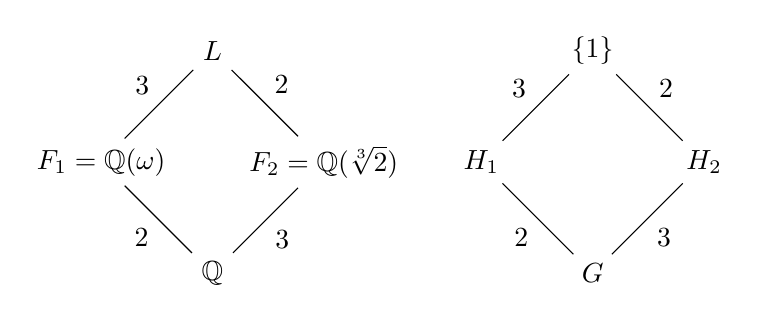
\begin{tikzpicture}[node distance = 2cm]
            \node (Q) {$\mathbb{Q}$};
            \node (F_1) [above left of=Q] {$F_1 = \mathbb{Q}(\omega)$};
            \node (F_2) [above right of=Q] {$F_2 = \mathbb{Q}(\sqrt[3]{2})$};
            \node (L) [above right of =F_1] {$L$};
            \node (H_1) [right of =F_2] {$H_1$};
            \node (1) [above right of =H_1] {$\{1\}$};
            \node (H_2) [below right of=1] {$H_2$};
            \node (G) [below right of =H_1] {$G$};

            \draw (Q) -- (F_1) node[midway,anchor=north east]{2}
                -- (L) node[midway, anchor=south east]{3}
                -- (F_2) node[midway, anchor = south west]{2}
                -- (Q) node[midway, anchor = north west]{3};
            \draw (G) -- (H_1) node[midway,anchor=north east]{2}
                -- (1) node[midway, anchor=south east]{3}
                -- (H_2) node[midway, anchor = south west]{2}
                -- (G) node[midway, anchor = north west]{3};
        \end{tikzpicture}
        \captionsetup{labelformat=empty}
    \caption{\hspace{6mm} Fields \hspace{35mm} Groups}
    \end{figure}

    This gives us a subfield lattice with a corresponding subgroup lattice, where each field is the fixed field of the corresponding group. The numbers on the edges correspond to the degrees of field extensions on the left and the indices of the subgroups on the right.
    \vspace{1mm}

    Since $|G|=6$, $G$ is isomorphic to either $C_6$ or $S_3$. Note that $F_2 / \mathbb{Q}$ is not normal, as $\omega \sqrt[3]{2} \not\in F_2$, so $H_2 = \text{Gal}(L/F_2)$ is not a normal subgroup. Hence $G$ is nonabelian, so $G \cong S_3$.

    Hence we have $H_2 \cong \{(12),e\}$ (by relabeling if necessary) and we must have $H_1 \cong A_3$. We have two other subgroups $\{(13), e\}$ and $\{(23),e\}$. There are the \textbf{conjugates} of $H_2$, so the corresponding subfields are $\{\sigma F_2 \mid \sigma \in G\}$, which are $\mathbb{Q}(\omega \sqrt[3]{2}), \mathbb{Q}(\omega^2 \sqrt[3]{2})$ (the conjugates of $\sigma(\sqrt[3]{2})$, $\sigma \in G$ are the roots of the minimal polynomial).

    So this describes all $F$ with $\mathbb{Q} \subset F \subset L$.
\end{example}

In fact, we could have seen at once that $G \cong S_3$:

Suppose $f \in K[T]$ is a separable polynomial, $x_1,\ldots,x_n$ are its roots in a splitting field $L$ (where $n=\text{deg}(f)$). Then $G = \text{Gal}(L/K)$ permutes the $\{x_i\}$ (as $f(\sigma x_i) = \sigma f(x_i) = 0$), and if $\sigma(x_i) = x_i ~\forall i$, then since $L = K(x_1,\ldots,x_n)$, $\sigma = \text{id}$. This gives an injective homomorphism $G \to S_n$.

So in the above example, we have a subgroup of $S_3$ of order $6$, so it must be
$S_3$.

\begin{defn}
    The subgroup $\text{Gal}(f/K) \subset S_n$ given by the image of $G$ is the \textbf{Galois group} of $f$ over $K$.
\end{defn}
\textbf{Note.} $[L:K] = |\text{Gal}(L/K)| = |\text{Gal}(f/K)|$, which is a subgroup of $S_n$, so it divides $n!$.

\vspace{1mm}

There exist several methods for determining the Galois group $\text{Gal}(f/K)$. Two useful results to know:
\begin{defn}
    A subgroup $G \subset S_n$ is \textbf{transitive} if $~\forall i,j \in \{1,2,\ldots,n\}, \exists \sigma \in G$ with $\sigma(i)=j$, i.e. $G$ only has one orbit.
\end{defn}
\begin{prop}
    $f$ is irreducible $\iff$ $\text{Gal}(f/K)$ is \textbf{transitive}.
\end{prop}
\begin{proof}
    Let $x$ be a root of $f$ in the splitting field $L$. Then its orbit under $G = \text{Gal}(f/K)$ is the set of roots of $m_{x,K}$ (by Theorem \ref{9.2}). As $m_{x,K} \mid f$, we have $m_{x,K} = f$ if and only if $f$ is irreducible. Furthermore, $m_{x,K} = f$ if and only if every root of $f$ is in the orbit of $x$, i.e. if and only if $G$ acts transitively on the roots of $f$.
\end{proof}
\textbf{Remark.} If $G$ is transitive, then by orbit-stabilizer theorem, $n \mid |G|$.

Recall from Section 2 that we defined the \textbf{discriminant}: if $f \in K[T]$ is monic and $f = \prod_{1\le i \le n}^{} (T-x_i)$ in a field $L$, then
\[
\text{Disc}(f) = \Delta^2 \in K,
\]
where $\Delta = \prod_{1\le i < j \le n}^{} (x_i-x_j)^2$. The discriminant is nonzero if and only if $f$ is separable.
\begin{prop}
    Let $L$ be a splitting field over $K$ and $G$ a Galois group for a monic separable polynomial $f \in K[T]$. Assume $\text{char}(K)\neq 2$. Then the fixed field of $G \cap A_n$ is $K(\Delta)$.
    \vspace{1mm}

    In particular, $\text{Gal}(f/K) \subset A_n$ if and only if $\text{Disc}(f)$ is a square in $K$.
\end{prop}

\begin{proof}
    \marginpar{03 Nov 2022, Lecture 13}

    $\pi \in S_n$, and $\pi$ has a sign $\pm 1$, where $$\prod_{1\le i<j\le n}^{} (T_{\pi(i)}-T_{\pi(j)})=\text{sgn}(\pi)\prod_{1\le i<j\le n}^{} (T_i-T_j).$$

    So if $\sigma \in G$, then $\sigma(\Delta) = \text{sgn}(\sigma)\Delta$. As $\Delta \neq 0$ and $\text{char}(K)\neq 2$, this implies that $\Delta \in K \iff G \in A_n$ and $\Delta$ lies in the fixed field $F$ of $G \cap A_n$. As $[F: K] = [G : G \cap A_n] = \begin{cases}
        1 &\text{ if } G \subset A_n \\
        2 &\text{ otherwise}
    \end{cases}$, we have $F = K(\Delta)$.
\end{proof}
\begin{example}
    Take $n=3$ and $f = T^3+aT+b = \prod_{i=1}^{3} (T-X_i)$. Then $x_3 = -x_1-x_2$, $a = x_1x_2 - (x_1+x_2)^2$ and $b=x_1x_2(x_1+x_2)$. Thus \[
    \text{disc}(f) = ((x_1-x_2)(2x_1+x_2)(x_1+2x_2))^2 = -4a^3 - 27b^2.
    \]
    So $\text{Gal}(f/K) \subset A_3 \iff -4a^3-27b^2$ is a square in $K$.
    \vspace{1mm}

    For example, take $f = T^3-21T - 7 \in \mathbb{Q}[T]$, which is irreducible. Then $\text{disc}(f)=4 \cdot 21^3 - 27 \cdot  7 ^2 = (27\cdot 7)^2$. So $\text{Gal}(f/\mathbb{Q}) \subset A_3$. As $f$ is irreducible, the Galois group is \textbf{transitive}. So $\text{Gal}(f/\mathbb{Q}) = A_3$.
\end{example}
This allows us to compute the Galois group of any cubic polynomial (of say $\text{char}(K)\neq2,3$).

\section{Finite fields}

Let $p$ be a prime and $\mathbb{F}_p = \mathbb{Z}/p\mathbb{Z}$. We aim to describe all finite fields of characteristic $p$ (i.e. finite extensions $F$ of $\mathbb{F}_p$) and their Galois theory. Recall that:
\begin{itemize}
    \item $|F|=p^n, [F : \mathbb{F}_p] = n$.
    \item $F^{\times}$ is cyclic and of order $p^n-1$.
    \item $\phi_p : F \to F$ by $x \mapsto x^p$ is an automorphism of $F$ (Frobenius).
\end{itemize}
\begin{theorem}\label{10.1}
    Let $n\ge 1$. Then there exists a field with $q=p^n$ elements. Any such field is a splitting field of the polynomial $f=T^q-T$ over $\mathbb{F}_p$. In particular, any two finite fields of the same order are isomorphic.
\end{theorem}
\begin{proof}
    Let $F$ be a field with $q=p^n$ elements. Then if $x \in F^{\times}, x^{q-1}=1$, so $~\forall x \in F, x^q = x$. So $f = \prod_{x \in F}^{} (T-x)$ splits into linear factors in $F$, and not in any proper subfield of $F$. So $F$ is a splitting field for $f$ over $\mathbb{F}_p$. By uniqueness of splitting fields, $F$ is unique up to isomorphism.
    \vspace{1mm}

    Conversely, given $n$, let $q=p^n$, let $L/\mathbb{F}_p$ be a splitting field for $f = T^q - T$ and let $F \subset L$ be the fixed field of $\phi_p^n : x \mapsto x^q$. So $F$ is the set of roots of $f= T^q-T$ in $L$. So $|F|=q$ (and $F=L$).
\end{proof}
\textbf{Notation.}  We write $\mathbb{F}_q$ for any finite field with $q$ elements. By Theorem \ref{10.1}, any two are isomorphic, although there is no "preferred" or "canonical" isomorphism.
\begin{theorem}
    $\mathbb{F}_{p^n}/\mathbb{F}_p$ is Galois, with Galois group cyclic of order $n$, generated by $\phi_p$ (the Frobenius automorphism).
\end{theorem}
\begin{proof}
    $T^{p^n}-T = \prod_{x \in \mathbb{F}_{p^n}}^{} (T-x)$ is separable, so $\mathbb{F}_{p^n}$ is Galois over $\mathbb{F}_p$ (as it is the splitting field of a separable polynomial). Let $G\subset \text{Gal}(\mathbb{F}_{p^n}/\mathbb{F}_p)$ be the subgroup generated by $\phi_p$. Then $\mathbb{F}_{p^n}^{G} = \{x \mid x^p = x\} = \mathbb{F}_p$. So by Galois correspondence, $G = \text{Gal}(\mathbb{F}_{p^n}/\mathbb{F}_p)$.
\end{proof}
\begin{theorem}
    $\mathbb{F}_{p^n}$ has a unique subfield of order $p^m$ for each $m \mid n$, and no others. If $m \mid n$, then $\mathbb{F}_{p^m} \subset \mathbb{F}_{p^n}$ is the fixed field of $\phi_p^m$.
\end{theorem}
\begin{proof}
    $\text{Gal}(\mathbb{F}_{p^n}/\mathbb{F}_n) \cong \mathbb{Z}/n\mathbb{Z}$. The subgroups of $\mathbb{Z}/n\mathbb{Z}$ are $m\mathbb{Z}/n\mathbb{Z}$ for $m \mid n$. So by Galois correspondence, the subfields of $\mathbb{F}_{p^n}$ are the fixed fields of these subgroups, i.e. the subgroups $\langle\phi^m \rangle$, which have degree equal to the indices $[\mathbb{Z}/n\mathbb{Z} : m \mathbb{Z}/ n\mathbb{Z}] = m$.
\end{proof}
\textbf{Remark.} If $m \mid n$, then $\text{Gal}(\mathbb{F}_{p^n}/\mathbb{F}_{p^m}) = \langle \phi_p^m\rangle$ with order $\frac{n}{m}$.
\begin{theorem}\label{10.4}
    Let $f \in \mathbb{F}_p[T]$ be separable of degree $n\ge 1$ whose irreducible factors have degrees $n_1,\ldots,n_r$ with $\sum_{}^{} n_i =n$. Then $\text{Gal}(f/\mathbb{F}_p) \subset S_n$ is cyclic, generated by an element of cycle type $(n_1,\ldots,n_r)$. In particular, $|\text{Gal}(f/\mathbb{F}_p)|=\text{lcm}(n_1,\ldots,n_r)$.
\end{theorem}
\textbf{Remark.} Cycle type $(n_1,\ldots,n_r)$ means that $\sigma$ is a product of disjoint cycles of lengths $n_i$.
\begin{proof}
    Let $L$ be a spliting field for $f$ over $\mathbb{F}_p$ and let the roots be $x_1,\ldots,x_n$. Then $\text{Gal}(L/\mathbb{F}_p)$ is cyclic and generated by $\phi_p$. As the irreducible factors of $f$ are the minimal polynomials of the $x_i$'s and the set of roots of the minimal polynomial of $x_i$ is the orbit of $\phi_p$ on $x_i$, the cycle type of $\phi_p$ is $(n_1,\ldots,n_r)$. The order of such a permutation is the LCM of $\{n_i\}$.
\end{proof}

\marginpar{05 Nov 2022, Lecture 14}

\begin{theorem}[Reduction mod $p$]\label{10.5}
    Suppose $f \in \mathbb{Z}[T]$ is monic and separable, $p$ is a prime, and $n = \text{deg}(f)\ge 1$. Suppose that the reduction $\overline{f} \in \mathbb{F}_p[T]$ of $f$ mod $p$ is also separable. Then
    \[
    \text{Gal}(\overline{f}/\mathbb{F}_p) \subset \text{Gal}(f/\mathbb{Q})
    \]
    as subgroups of $S_n$.
\end{theorem}
\begin{cor}\label{10.6}
    With the same assumptions as in Theorem \ref{10.5}, suppose that $\overline{f}=g_1\ldots g_r$ with $g_i \in \mathbb{F}_p[T]$ irreducible of degree $n_i$. Then $\text{Gal}(f/\mathbb{Q})$ contains an element of cycle type $(n_1,\ldots,n_r)$.
\end{cor}
\begin{proof}
    Combine Theorem \ref{10.4} and Theorem \ref{10.5}.
\end{proof}
\begin{example}
    $f = T^4 - 3T + 1$.
    \begin{itemize}
        \item If $p=2$, then $f = T^4+T+1 \pmod{2}$, which is irreducible (as it is not divisible by $T^2+T+1$, the only irreducible polynomial of degree 2).
        \item If $p=5$, then $f=(T+1)(\underbrace{T^3-T^2+T+1}_{\text{irreducible}})$.
    \end{itemize}
    So by Corollary \ref{10.6}, we see that $\text{Gal}(f/\mathbb{Q})=G$ contains a 4--cycle and a 3--cycle, so $|G|$ is divisible by $12$ and so is either $S_4$ or $A_4$ (as it is the unique subgroup of $S_4$ of order 12). But $4$--cycles are odd, so $G = S_4$.
\end{example}
\textbf{Remark.} If $\overline{f}$ is separable, then $\text{Disc}(\overline{f}) \neq 0$, so $p \nmid \text{Disc}(f)$, i.e. $f$ is separable.
\vspace{1mm}


\textbf{Remark.} If $f$ is separable, then $\overline{f}$ will be separable for all but the finite set $\{p \mid \text{Disc}(f)\}$. So we have lots of values of $p$ to try.
\vspace{1mm}


\textbf{Remark.} The meaning of $\text{Gal}(\overline{f}/\mathbb{F}_p) \subset \text{Gal}(f/\mathbb{Q})$: The identification of $\text{Gal}(f/\mathbb{Q})$ with a subgroup of $S_n$ depends on fixing a labeling/ordering of the roots. Taking a different ordering conjugates $\text{Gal}(f/\mathbb{Q})$ inside $S_n$ (by the permutation giving the reordering). So the above statement really means that $\text{Gal}(\overline{f}/\mathbb{F}_p)$ is conjugate to a subgroup of $\text{Gal}(f/\mathbb{Q})$.
\vspace{1mm}

There exist at least two proofs of Theorem \ref{10.5}. One of the proofs is difficult to understand, and will be posted on the Moodle page. The other proof has a flavor of algebraic number theory, but is self-contained and we present it here:
\begin{proof}[Proof of Theorem \ref{10.5} (non-examinable)]
    Let $L=\mathbb{Q}(x_1,\ldots,x_n)$ be the splitting field for $f = \prod_{}^{} (T-x_i)$ of degree $N=[L:\mathbb{Q}]$. Consider $R = \mathbb{Z}[x_1,\ldots,x_n]$. As $f(x_i)=0$, $f$ is monic and every element of $R$ is a $\mathbb{Z}$--linear combination of $x_1^{\alpha_1},\ldots,x_n^{\alpha_n}$ for $0\le \alpha_i\le N$. So $R$ is finitely generated as an abelian group. As $R \subset L \cong \mathbb{Q}^N$, we must have $R \cong \mathbb{Z}^M$ for $M\le N$. (In fact, $M=N$, but we don't prove that here).
    \vspace{1mm}

    Now consider $\overline{R}=R/pR$, which has $p^M$ elements. Let $\overline{P}$ be a maximal ideal of $\overline{R}$, corresponding to an ideal $P$ of $R$ containing $pR$. Then $F = R/pR \cong \overline{R}/\overline{P}$ (by the isomorphism theorems) is a finite field with of characteristic $p$, so say it has $p^d$ elements. $F = \mathbb{F}_p(\overline{x_1},\ldots,\overline{x_n})$, where $\overline{x_i}=x_i+P \in F$ and $\overline{f}=\prod_{n=1}^{} (T-\overline{x_i})$. As $\overline{f}$ is separable, the $\overline{x_i}$ are distinct, so $F$ is a splitting field for $\overline{f}$.
    \vspace{1mm}

    $G = \text{Gal}(f/\mathbb{Q})$ takes $R$ to itself (as it permutes the $x_i$). Let $H \subset G$ be the stabilizer of $P$, i.e. $\{\sigma \in G \mid \sigma P = P\}$. Then $H$ acts on $R/P = F$, permuting the $\overline{x_i}$'s in the same way as it permutes the $x_i$'s. So we have an injective homomorphism $H \hookrightarrow \text{Gal}(f/\mathbb{F}_p)$. It is enough to show that this is an isomorphism. Let $\{P_1,\ldots,P_r\}$ be the orbit of $G$ under $G$ ($P_i= \sigma P$ for some $\sigma \in G$). $P_i$ are all maximal ideals (because $P$ is), $R/P_i \cong R/P$ has $p^d$ elements as well. As the $P_i$ are maximal, $P_i+P_j = R$ if $i\neq j$. So by Chinese Remainder Theorem, $R/(P_1 \cap \ldots \cap P_r) \cong R/P_1 \times \ldots \times R/P_r$. As $p \in P_i$, $pR \subset P_1 \cap \ldots \cap P_r$, so \[
    p^N \ge p^M = |R/pR| \ge |R/(P_1 \cap \ldots \cap P_r)| = \prod_{i=1}^{r} |R/P_i| = p^{rd},
    \]
    so $N \ge rd$. By the Orbit-Stabilizer Theorem, $r=[G:H] = \frac{N}{|H|}$, and because $H \hookrightarrow \text{Gal}(F/\mathbb{F}_p)$ (i.e. $H$ injects into $\text{Gal}(F/\mathbb{F}_p)$), we have $|H|\le d$ if and only if the above map is an isomorphism. So $N\le rd$. Hence $N=rd$, so $H \cong \text{Gal}(\overline{f}/\mathbb{F}_p)$.
\end{proof}
\textbf{Remark.} If $\text{Gal}(f/\mathbb{Q})$ contains an element of cycle type $(n_1,\ldots,n_r)$, then it is a (hard!) fact that exist infinitely many primes such that $\overline{f}$ factors into irreducibles of degrees $n_1,\ldots,n_r$. This is called Chebotarov's density theorem -- it is a generalization of Dirichlet's theorem on primes in arithmetic progressions. This might be proved in II Number Fields.

\section{Cyclotomic extensions}
We consider polynomials of the form $T^n-1$ (and later $T^n-a$).

\begin{lemma}\label{11.1}
    Let $C$ be a cyclic group of order $n \ge 2$ (written multiplicatively). If $a \in \mathbb{Z}$ and $(a,n)=1$, then the map $[a] : C \to C$ by $[a]g=g^a$ is an \textbf{automorphism} of $C$, and the map $$(\mathbb{Z}/n\mathbb{Z})^{\times} \to \text{Aut}(c), a \mapsto [a]$$ is an isomorphism.
\end{lemma}
\begin{proof}
    $[a]$ is obviously a homomorphism, and it is an automorphism since $\exists b$ with $ab \equiv 1 \pmod{n}$. So we have an injective map $(\mathbb{Z}/n\mathbb{Z})^{\times} \hookrightarrow \text{Aut}(C)$ by $a \mapsto [a]$, which is obviously a homomorphism. If $\phi \in \text{Aut}(C)$ and $g$ is a generator of $C$, then $\phi(g)=g^a$ for some $a \in (\mathbb{Z}/n\mathbb{Z})^{\times}$, so $\phi = [a]$, so we have an isomorphism.
\end{proof}

\marginpar{08 Nov 2022, Lecture 15}

Let $K$ be a field and $n\ge 1$. Define $\mu_n(K)= \{x \in K \mid x^n=1\}$, the group of $n^{\text{th}}$ roots of unity in $K$ under multiplication. This is finite, hence cyclic (by Proposition \ref{3.5}), hence of order dividing $n$.
\vspace{1mm}

We say $\zeta \in \mu_n(K)$ is a \textbf{primitive} $n^{\text{th}}$ root of 1 if $\zeta$ has order exactly $n$ in $K^{\times}$. Such a $\zeta$ exists if and only if $\mu_n(K)$ has order $n$ (and then $\zeta$ is a generator for $\mu_n(K)$). In particular, $f=T^n-1$ has $n$ distinct roots, so it is separable.
\vspace{1mm}

In general, $T^n-1=f$ is separable $\iff (f,f')=1$ and since $f'=nT^{n-1}$, this holds if and only if $n\cdot 1_K \neq 0$.
\vspace{1mm}

\textbf{Important:} From now on, until the end of the section, assume that either $\text{char}(K)=0$ or $\text{char}(K)=p>0$ and $p \nmid n$ (in other words, that $f=T^n-1$ is separable).
\vspace{1mm}

Let $L/K$ be a splitting field for $T^n-1$ and let $G=\text{Gal}(L/K)$ ($L/K$ is Galois as $f$ is separable). Then $|\mu_n(L)|=n$, so there exists a primitive $n^{\text{th}}$ root of 1, $\zeta=\zeta_n \in L$. $L/K$ is called a \textbf{cyclotomic extension}.

\begin{prop}\label{11.2}
    \begin{enumerate}[(i)]
        \item $L=K(\zeta)$.
        \item There exists an injective homomorphism $\chi = \chi_n : G = \text{Gal}(L/K) \to (\mathbb{Z}/n\mathbb{Z})^\times$ such that if $\chi(\sigma)=a \pmod{n}$, then $\sigma(\zeta)=\zeta^a$. In particular, $G$ is abelian.
        \item $\chi$ is an isomorphism if and only if $G$ acts transitively on the set of primitive roots of unity in $L$. ($\chi$ is called the \textbf{cyclotomic character}).
    \end{enumerate}
\end{prop}
\begin{proof}
    \begin{enumerate}[(i)]
        \item $\mu_n(L)=\langle\zeta \rangle$, so the roots of $f=T^n-1$ are the powers of $\zeta$, so $L=K(\{\zeta^a\})=K(\zeta)$.
        \item Consider the action on $G$ on $L$. It permutes the roots $\mu_n(L)$ and if $\zeta,\zeta' \in \mu_n(L)$, $\sigma \in G$, then $\sigma(\zeta \zeta') = \sigma(\zeta)\sigma(\zeta')$, so $\sigma$ acts as an automorphism on $\mu_n(L)$, and $\sigma(\zeta_n)=\zeta_n \iff \sigma=\text{id}$. So we have an injective homomorphism $G \hookrightarrow \text{Aut}(\mu_n(L)) \cong (\mathbb{Z}/n\mathbb{Z})^\times$ by Lemma \ref{11.1}.
        \item $\zeta_n^a$ is primitive if and only if $(a,n)=1$, so the set of primitive $n^{\text{th}}$ roots of 1 is the set $\{\zeta^a \mid a \in (\mathbb{Z}/n\mathbb{Z})^\times\}$ which by (ii) equals the orbit of $\zeta$ under $G$. Hence the result follows.
    \end{enumerate}
\end{proof}
\begin{example}
    If $K=\mathbb{Q}$, take $L=\mathbb{Q}(e^{\frac{2 \pi i}{n}})$. What is the minimal polynomial of $e^{2\pi/n}$?
\end{example}
\begin{defn}
    Let $K$ be a field satisfying the above earlier hypothesis. The $n^{\text{th}}$ \textbf{cyclotomic polynomial} is $$\Phi_n(T)=\prod_{a \in (\mathbb{Z}/n\mathbb{Z})^\times}^{} (T-\zeta_n^a)$$ (where the roots are the primitive $n^{\text{th}}$ roots of 1 in $L$, the splitting field for $T^n-1$). 
\end{defn}
As $G$ permutes the primitive $n^{\text{th}}$ roots of 1 in $L$, $\Phi_n \in L^G[T] = K[T]$. So we can rephrase (iii) in Proposition \ref{11.2} as saying that $\chi$ is surjective if and only if $\Phi_n \in K[T]$ is irreducible.
\vspace{1mm}

$\Phi_n$ doesn't really depend on $K$. In fact, $x \in L$ satisfies $x^n=1$ if and only if $x$ is a primitive root of 1 for some (unique) $d \mid n$. So $$T^n-1 = \prod_{d \mid n}^{} \Phi_d \implies \Phi_n = \frac{T^n-1}{\prod_{d \mid n, d\neq n}^{} \Phi(d)}.$$
This gives an inductive definition of $\Phi_n$ and we see that $\Phi_n$ is the image in $K[T]$ of a polynomial in $\mathbb{Z}[T]$ which doesn't depend on $K$.

For example, $\Phi_p = \frac{T^p-1}{T-1}=T^{p-1}+T^{p-2}+\ldots+T+1$, $\Phi_1 = T-1$, and $\Phi_{p^n} = \frac{T^{p^n}-1}{T^{p^{n-1}}-1} = \Phi_p(T^{p^{n-1}})$. Also, $\text{deg}(\Phi_n) = |(\mathbb{Z}/n\mathbb{Z})^\times|=\phi(n)$, the Euler phi function.
\vspace{1mm}

We have two special cases:
\begin{theorem}[Irreducibility of cyclotomic polynomials]
    Let $K=\mathbb{Q}$. Then $\chi_n$ is an isomorphism for every $n>1$. In particular, $[\mathbb{Q}(\zeta_n):\mathbb{Q}]=\phi(n)$, and $\Phi_n$ is irreducible over $\mathbb{Q}$.
\end{theorem}
\begin{proof}
    By Proposition \ref{11.2}, these statements are all equivalent. So it suffices to prove that $\Phi_n$ is irreducible over $\mathbb{Q}$. If $n$ is prime (or a prime power), we can prove this using Eisenstein's criterion, but this doesn't work in the general case.

    $\chi_n$ is an isomorphism if for all primes such that $(p,n)=1$, the class of $p \in (\mathbb{Z}/n\mathbb{Z})^\times$ lies in the image of $\chi$ (because we can factor $a$ with $(a,n)=1$ as a product of such primes).

    Let $f$ be the minimal polynomial of $\zeta$ over $\mathbb{Q}$, and $g$ the minimal polynomial of $\zeta^p$ over $\mathbb{Q}$. If $f=g$, then $\zeta^a$ lies in the orbit of $G$ on $\zeta \implies p$ is in the image of $\chi$ and we're done.

    If $f\neq g$, then $(f,g)=1$ and they both divide $T^n-1$, so $fg \mid T^n-1$. As $\zeta$ is a root of $g(T^p)$, $f \mid g(T^p)$. Reduce this modulo $p$ to get $\overline{f} = f \pmod{p} \in \mathbb{F}_p[T]$ that divides $g(T^p) = \overline{g}(T)^p$ (as we're in characteristic $p$) and as both $\overline{f}$ and $\overline{g}$ divide $T^n-1 \in \mathbb{F}_p[T]$, which is separable (as $p \nmid n$), this implies $\overline{f} \mid \overline{g}$. Hence $\overline{f}^2 \mid \overline{f}\overline{g} \mid T^n-1$, contradicting separability of $T^n-1$. Hence this case is impossible and we're done.
\end{proof}
So the minimal polynomial of $e^{2\pi/n}$ over $\mathbb{Q}$ is $\Phi_n(T)$.
\vspace{1mm}

\marginpar{10 Nov 2022, Lecture 16}

Now we consider $K=\mathbb{F}_p$. Recall that $\phi_p \in G$ is the map $\phi(x)=x^p$, the Frobenius map, and $\phi_p$ generates $G$.
\begin{prop}
    Let $K=\mathbb{F}_p$ and $(n,p)=1$. Then
    \begin{enumerate}[(i)]
        \item $\chi_n : G \to \langle \phi \rangle \subset (\mathbb{Z}/n\mathbb{Z})^\times$ (the subgroup generated by a residue class mod $p$) and $\chi_n(\phi_p)=p \pmod{n}$.
        \item $[L:K]=r$, the order of $p$ mod $n$.
        \item $\phi_p$ has cycle type $(r,\ldots,r)$ as a permutation of the roots of $\Phi_n$.
    \end{enumerate}
\end{prop}
\begin{proof}
    $\phi_p(\zeta)=\zeta^p$, and $L=K(\zeta)$, so $\chi(\phi_p)=p$, hence $\chi_n(G)=\langle p \rangle$ and $[L:K] = |G| = |\langle p \rangle| =$ the order of $p$ mod $n$. This implies (i) and (ii).
    \vspace{1mm}
    
    If $(a,n)=1$, then when is $\phi_p^k(\zeta^a)=\zeta^a \iff \phi_p^k(\zeta)=\zeta \iff r \mid k$. So the orbits of $\phi_p$ on $\{\zeta^a \mid (a,n)=1\}$, i.e. the set of roots of $\Phi_n$, all have length $r$, which implies (iii). 
\end{proof} 
\textbf{Remarks.}
\begin{itemize}
    \item This almost gives another proof of the irreducibility of $\Phi_n$ over $\mathbb{Q}$. By the reduction mod $p$ theorem, $\text{Gal}(\Phi_n/\mathbb{Q}) \supset \text{Gal}(\Phi_n/\mathbb{F}_p)$ as subgroups (up to conjugacy) of the symmetric group $S_{\phi(n)}$. It is not hard to show that $\chi_n(\text{Gal}(\Phi_n/\mathbb{Q})) \supset \chi_n(\text{Gal}(\Phi_n/\mathbb{F}_p)) = \langle p \rangle$. As this holds for all $p \nmid n$, we get $\chi(\text{Gal}(\Phi_n/\mathbb{Q}))=(\mathbb{Z}/n\mathbb{Z})^\times$.
    \item (iii) implies that the factorization of $\Phi_n$ over $\mathbb{F}_p$ is $\prod_{}^{} (\text{irred. of degree }r)$, which only depends on the order of $p$ mod $n$. For a general polynomial $f \in \mathbb{Z}[T]$, the factorization of $f$ mod $p$ doesn't follow any obvious pattern. Trying to answer this question is a part of the Langlands Program, and the case where there is a congruence pattern is when $\text{Gal}(f/\mathbb{Q})$ is abelian (''Class Field Theory'').
\end{itemize}

\textbf{Application 1.} Quadratic reciprocity.

Recall that if $p$ is an odd prime and $a \in \mathbb{Z}$ with $(a,p)=1$, then the Legendre symbol is defined as $\left( \frac{a}{p} \right) = \begin{cases}
    1 &\text{ if } a \text{ is a square mod }p.\\
    -1 &\text{ if not.}
\end{cases}$
\vspace{1mm}

Euler's formula says $\left( \frac{a}{p} \right) \equiv a^{\frac{p-1}{2}} \pmod{p}$. Now let $q \neq p$ be another odd prime and say $n=q$. Then $L=K(\zeta_q)$ is a splitting field for $f=T^q-1 = (T-1)\Phi_q$. So on roots of $f$ in $L$, the Frobenius map $\phi_p$ has cycle type $(1,r,\ldots,r)$ with $\frac{q-1}{r}$ $r$--cycles. 

So its sign is $\text{sgn}(\phi_p) = (-1)^{r-1}\cdot (q-1)/r = (-1)^{(q-1)/r}$ and $2 \mid \frac{q-1}{r} \iff r \mid \frac{q-1}{2} \iff p^{\frac{q-1}{2}} \equiv 1 \pmod{q}$. So $\text{sgn}(\phi_p) = \left( \frac{p}{q} \right)$ by Euler's formula. But as $G = \langle \phi_p \rangle$, $\text{sgn}(\phi_p) = 1 \iff G \subset A_q$ (for $q=\text{deg}(f)$). But this holds if and only if $\text{Disc}(f)$ is a square in $\mathbb{F}_p$.
\vspace{1mm}

A lemma we prove on Example Sheet 3:
\begin{lemma}
    Let $f=\prod_{}^{(T-x_i)}$ over any field. Then $$\text{Disc}(f)= (-1)^{d(d-1)/2}\prod_{}^{} f'(x_i)$$ for $d=\text{deg(f)}$.
\end{lemma}

So in our case, $f=T^q-1 = \prod_{a=0}^{q-1} (T-\zeta_q^a)$ and $f'=qT^{q-1}$. So as $q$ is odd, 
\begin{align*}
    \text{Disc}(f) = (-1)^{q(q-1)/2} \prod_{a=0}^{q-1} q (\zeta_q^a)^{q-1} = (-1)^{(q-1)/2}q^q \zeta_q^{q-1} = (-1)^{\frac{q-1}{2}}q^q.
\end{align*}
So $\left( \frac{p}{q} \right)  = \left( \frac{\text{Disc}(f)}{p} \right) =\left( \frac{(-1)^{(q-1)/2}q}{p} \right) = \left( \frac{q}{p} \right) (-1)^{(p-1)(q-1)/4}$, which gives quadratic reciprocity.

This is essentially Stickelberger's proof, although he didn't have Galois theory.
\vspace{1mm}

\textbf{Application 2.} Construction of regular polygons.
\vspace{1mm}

Ruler--and--compass construction of a regular $n$--gon ($n\ge 3$) is equivalent to constructing $\cos(\frac{2\pi}{n})$.

\begin{theorem}[Gauss]
    A regular $n$--gon is constructible if and only if $n$ is a power of 2 times a product of distinct primes, each of the form $2^{2^k}+1$.
\end{theorem}
\textbf{Remark.} When is $F_k=2^{2^k}+1$ prime? (These are called Fermat numbers). We have $F_1=5,F_2=17,F_3=257,F_4=65537$, which are all prime. Fermat conjectured that all $F_k$ are prime. However, Euler showed that $F_5 = 641 \cdot 6700417$. Since then, many $F_k$'s are known to be composite and none prime for $k>4$.

\marginpar{12 Nov 2022, Lecture 17}

\begin{proof}
    Recall $x \in \mathbb{R}$ is constructible $\iff$ $\exists $ fields $\mathbb{Q}=K_0 \subset K_1 \subset \ldots \subset K_m \ni x$ and $[K_{i+1}:K_i]=2 ~\forall i$. In particular, a necessary condition is that $\text{deg}_\mathbb{Q}(x)$ is a power of 2. In our case, $x=\cos(\frac{2\pi}{n}) = \frac{1}{2}(\zeta_n+\zeta_n^{-1})$ for $\zeta_n = e^{2\pi i/n}$, so $\zeta_n^2 - 2x \zeta_n + 1 =0.$

    We have $x \in \mathbb{R}, \zeta_n \neq \mathbb{R}$, so $[\mathbb{Q}(\zeta_n):\mathbb{Q}(x)]=2$. So if $x$ is constructible, then $[\mathbb{Q}(\zeta_n):\mathbb{Q}]$ is a power of 2, but if $n=\prod_{i=1}^{r} p_i^{e_i}$, then
    \[
    [\mathbb{Q}(\zeta_n):\mathbb{Q}] = \phi(n) = \prod_{i}^{} p_i^{e_i-1}(p-1).
    \]
    So this is a power of 2 if and only if for all odd $p_i$, $e_i=1$ and $p_i-1$ is a power of 2.
    \begin{lemma}
        If $m$ is a positive integer such that $2^m+1$ is prime, then $m$ has to be a power of 2.
    \end{lemma}
    \begin{proof}
        $2^{qr}+1 = (2^r+1)(2^{qr-r}+2^{qr-2r}+\ldots+1)$ if $q$ is odd.
    \end{proof}
    So we conclude that $\phi(n)$ is a power of 2 if and only if $n$ is of the required form, so $x$ being constructible implies $n$ is of the required form.
    \vspace{1mm}
    
    For the other direction, suppose $\phi(n)=2^m$. Then $\mathbb{Q}(\zeta_n)/\mathbb{Q}$ is Galois, with Galois group $G \cong (\mathbb{Z}/n\mathbb{Z})^\times$ and $|G|=2^m$. Observe that there exist subgroups $G = H_0 \supset H_1 \supset H_2 \supset \ldots \supset H_n = \{e\}$ such that $[H_i:H_{i+1}]=2 ~\forall i$.

    Indeed, as $2 \mid |G|$, $\exists \sigma \in G$ of order 2 (assuming $G \neq \{e\}$). Now take $H_{m-1} = \langle \sigma \rangle$. Then $G/H_{m-1}$ contains  a subgroup of order 2 by the same argument, which we call $H_{m-2}/H_{m-1}$. Continue this way to construct all $H_i$. Then $K_i = \mathbb{Q}(\zeta_n)^{H_i}$ satisfy $[K_{i+1}:K_i]= [H_i : H_{i+1}]=2$, so we're done.
\end{proof}

\section{Kummer extensions}

Let $L=K(x)$, $x^n=a \in K$ (not necessarily $a=1$). We know these extensions are not necessarily Galois, for example $\mathbb{Q}(\sqrt[3]{2})/\mathbb{Q}$ is not Galois.

Let us first prove a result of independent interest.
\begin{theorem}[Linear independence of field embeddings]\label{12.1}
    Let $K,L$ be fields and let $\sigma_1,\ldots,\sigma_n : K \hookrightarrow L$ be distinct field homomorphisms. If $y_1,\ldots,y_n \in L$ such that $\forall x \in K$, $y_1\sigma_1(x) + \ldots + y_n \sigma_n(x)=0$, then $y_i=0 ~\forall i$.

    In other words, $\sigma_1,\ldots,\sigma_n$ are $L$--linearly independent elements of the set of functions $K \to L$, which is an $L$--vector space.
\end{theorem}

This is the special case $G=K^{\times}$ of a theorem in II Representation Theory:
\begin{theorem}[Linear independence of characters]
    For $G$ a group, $L$ a field, $\sigma_1,\ldots,\sigma_n : G \to L^{\times}$ group homomorphisms, we have that $\sigma_1,\ldots,\sigma_n$ are linearly independent over $L$.
\end{theorem}
\begin{proof}
    Induction on $n$. $n=1$ is clear.

    Now suppose that $n>1$ and we have elements $y_1,\ldots,y_n \in L$ such that $~\forall g \in G$, $y_1 \sigma_1(g) + \ldots + y_n \sigma_n(g) = 0 ~(\star).$ 

    $\exists h \in G$ such that $\sigma_1(h) \neq\sigma_n(h)$. As $\sigma_i$ are homomorphisms, substitute $hg$ into $(\star)$ and we get \[
    y_1 \sigma_1(h)\sigma_1(g) + \ldots y_n \sigma_n(h) \sigma_n(g).
    \]
    Multiply $(\star)$ by $\sigma_n(h)$ and subtract to get \[
    y_1' \sigma_1(g) + \ldots + y_{n-1}' \sigma_{n-1}(g) = 0,
    \]
    where $y_i'=y_i(\sigma_i(h)-\sigma_n(h))$. As $\sigma_1(h) \neq \sigma_n(h)$, $y_1=0$. Then $(\star)$ is a linear dependence between $\sigma_2,\ldots,\sigma_n$, hence by induction, $y_2=\ldots=y_n=0$.
\end{proof}
Assume now that $n>1$ and $n\cdot 1_K \neq 0$.
\begin{theorem}\label{12.3}
    Assume $K$ contains a primitive $n^{\text{th}}$ root $\zeta=\zeta_n$ of 1. Suppose $L/K$ is an extension with $L=K(x)$, $x^n=a \in K^{\times}$. Then
    \begin{enumerate}[(i)]
        \item $L/K$ is a splitting field for $f(T)=T^n-a$, and it is Galois with cyclic Galois group.
        \item $[L:K]$ is the least $m\ge 1$ such that $x^m \in K$.
    \end{enumerate}
\end{theorem}
\begin{proof}
    (i): As $\mu_n(K) = \{\zeta_n^i \mid 0\le i<n\}$ has $n$ elements, $f$ has $n$ distinct roots $\{\zeta_i x\}$ in $L$. So $L/K$ is a splitting field for the separable polynomial $f$, so it is Galois.

    Let $\sigma \in \text{Gal}(L/K) = G$. Then $f(\sigma(x))=0$, so $\sigma(x) = \zeta^i x$ for some $i$ which is unique mod $n$. Define a map $\Theta : G \to \mu_n(K)=\{\zeta^i\} \cong \mathbb{Z}/n\mathbb{Z}$ by $\Theta(\sigma) = \frac{\sigma(x)}{x}$. The claim is that this is a homomorphism: let $\sigma, \tau \in G$, then as $\zeta \in K$, $\tau(\Theta(\sigma))=\Theta(\sigma)$, so \[
    \Theta(\tau \sigma) = \frac{\tau \sigma(x)}{x} = \tau\left(\frac{\sigma(x)}{x}\right)  \frac{\tau(x)}{x} = \tau(\Theta(\sigma))\Theta(\tau)=\Theta(\sigma)\Theta(\tau).
    \]
    So $\Theta$ is a homomorphism, and $\Theta(\sigma)=1 \iff \sigma(x)=x \iff \sigma=\text{id}$, hence $\Theta$ is injective. So $G$ is isomorphic to a subgroup of a cyclic group, hence cyclic.
    \vspace{1mm}
    
    (ii): If $m\ge 1$, since $L/K$ is Galois,
    \begin{align*}
        &x^m \in K \iff ~\forall \sigma \in G, \sigma(x^m)=x^m \iff\\
        &\iff ~\forall \sigma \in G,\Theta(g)^m = 1 \iff |G|=[L:K] \text{ divides }m.
    \end{align*}
\end{proof}
\marginpar{15 Nov 2022, Lecture 18}
\begin{cor}
    Assume $K$ contains a primitive $n^{\text{th}}$ root of unity and let $a \in K^\times$. Then $f=T^n-a$ is irreducible in $K[T]$ if and only if $a$ is not a $d^{\text{th}}$ power in $K$ for any $1 \neq d \mid n$.
\end{cor}
\begin{proof}
    Let $L=K(x)$ for $x^n=a$. The minimal polynomial of $a$ divides $f$, so $f$ is irreducible $\iff |G|=[L:K]=n$. Suppose $n=md$ for $d \neq 1$. Then $a$ is a $d^{\text{th}}$ power in $K$ if and only if $x^m \in K$ (as $\zeta_n \in K$), which holds if and only if $|G| \mid m$.
\end{proof}
\textbf{Remark.} This doesn't hold in general if $\zeta_n \not\in K$, e.g. take $K=\mathbb{Q}$ and the polynomial $T^4+4$.
\vspace{1mm}

\textbf{Terminology.} Extensions of the form $L=K(\sqrt[n]{a})$, where $\zeta_n \in K$ are called \textbf{Kummer extensions}. 
\begin{example}
    $n=2, \text{char}(K)\neq 2$ and $\zeta_2 = -1 \in K$. Then $K(\sqrt{a})/K$ is quadratic if $a \not\in (K^\times)^2$ (i.e. $a$ is not a square). Conversely, every quadratic extension $L/K$ is $L=K(\sqrt{a})$ for some $a$ (by an example sheet question).
\end{example}
For general $n$ we have a converse to the above theorem:
\begin{theorem}\label{12.5}
    Suppose $K$ contains $\zeta$, a primitive $n^{\text{th}}$ root of $1$ ($n>1$). Let $L/K$ be Galois with $\text{Gal}(L/K)$ cyclic of order $n$. Then $L=K(\sqrt[n]{a})$ for some $a \in K^\times$.
\end{theorem}
\begin{proof}
    Let $G=\text{Gal}(L/K)=\{\sigma^i \mid 0\le i<n\}$. For $y \in L$, let $$x=R(y)=y + \zeta ^{-1}\sigma(y) + \ldots + \zeta^{-(n-1)}\sigma^{n-1}(y) = \sum_{j=0}^{n-1} \zeta^{-j}\sigma^j(y) \in L,$$
    a \textbf{Lagrange resolvent}. Then $$\sigma(x)=\sum_{j=0}^{n-1} \zeta^{-j}\sigma^{j+1}(y)=\sum_{j=0}^{n-1} \zeta^{1-j}\sigma^{j}(y) = \zeta x.$$ 
    Thus $\sigma(x^n)=x^n$, i.e. $x^n \in K$. By Theorem \ref{12.1} with $\{\sigma_i\} = \{1,\sigma,\ldots,\sigma^{n-1} : L \to L\}$, there exists $y$ such that $x\neq 0$. As $\sigma^i(x)=\zeta^i x$, the $\sigma^i(x)$ are distinct, so $\text{deg}_K(x)=n$ and so $L=K(x)$.
\end{proof}
\begin{example}
    Suppose $L/\mathbb{Q}$ has degree 3 and is Galois. Then as $\zeta_3 \not\in \mathbb{Q}$, this is not a Kummer extension.
\end{example}

\section{Trace and norm}
Let $L/K$ be an extension of degree $n$, so $L$ is an $n$--dimensional $K$--vector space. For $x \in L$, the map 
\begin{align*}
    &U_x : L \to L \\
    &U_x(y) = xy
\end{align*}
is obviously $K$--linear (as it is $L$--linear). So it has a characteristic polynomial, determinant, and trace.
\begin{defn}
    The \textbf{trace} and \textbf{norm} of $x$ (relative to $L/K$) are defined as 
    \begin{align*}
        &\text{Tr}_{L/K}(x) = \text{tr }U_x \\
        &N_{L/K}(x)=\det U_x.
    \end{align*}
    We will sometimes write $\text{tr}_K$, $\det_K$ if it is important to know the base field $K$.
    \vspace{1mm}
    
    The \textbf{characteristic polynomial} of $x$ is 
    \begin{align*}
        f_{x,L/K} = (\text{char. poly. of }U_x)= {\det}_K(t I - U_x).
    \end{align*}
    Explicitly, let $e_1,\ldots,e_n$ be a basis for $L/K$. Then there exists a unique matrix $A=(a_{ij})$ such that $x e_i = \sum_{j}^{} a_{ji}e_j$, and then $\text{Tr}_{L/K}(x)=\text{tr}(A)$, etc.
\end{defn}
\begin{example}
    Let $\mathbb{Q}(\sqrt{d})/\mathbb{Q}$ be quadratic with basis $\{1,\sqrt{d}\}$. Let $x=a+b\sqrt{d}$. Then \[
    A = \begin{pmatrix} a & bd \\ b & a \end{pmatrix}
    \] as $x \cdot 1 = a \cdot 1 + b \cdot  \sqrt{d}$ and $x \cdot \sqrt{d} = bd \cdot 1 + a \cdot \sqrt{d}$.
    \vspace{1mm}
    
    We hence find $\text{Tr}_{L/K}(x)=2a, N_{L/K}(x)=a^2-db^2$.
\end{example}
\begin{example}
    If we take $\mathbb{C}/\mathbb{R}$ with basis $\{1,i\}$, then the matrix of $U_{x+iy}$ is $\begin{pmatrix} x & -y\\y & x \end{pmatrix}$, which is the usual representation of complex numbers using $2\times 2$ real matrices (think Cauchy--Riemann).
\end{example}
\begin{lemma}\label{13.1}
    Take $x \in L, a \in K$ with $n = [L:K]$. Then
    \begin{enumerate}[(i)]
        \item $\text{Tr}_{L/K}(x+y) = \text{Tr}_{L/K}(x) + \text{Tr}_{L/K}(y)$ and $N_{L/K}(xy) = N_{L/K}(x) N_{L/K}(y)$.
        \item $N_{L/K}(x)=0 \iff x=0$.
        \item $\text{Tr}_{L/K}(1)=n, N_{L/K}(1)=1$.
        \item $\text{Tr}_{L/K}(ax)=a \text{Tr}_{L/K}(x)$ and $N_{L/K}(ax)=a^n N_{L/K}(x)$ (so $\text{Tr}_{L/K}$ is $K$--linear and $N_{L/K}: L^\times \to K^\times$ is a homomorphism).
    \end{enumerate}
\end{lemma}
\begin{proof}    
    For (ii), $N_{L/K}(x) = \det(U_x) \neq 0 \iff U_x$ is invertible, which holds iff $x\neq0$.
    \vspace{1mm}
    
    All other properties follow from the corresponding properties of trace and determinant of matrices.
\end{proof}

\marginpar{17 Nov 2022, Lecture 19}

\begin{theorem}\label{13.2}
    Let $M/L/K$ be finite extensions. Then 
    \begin{align*}
        &\text{Tr}_{L/K}(\text{Tr}_{M/L}(x)) = \text{Tr}_{M/K}(x) \\
        &N_{L/K}(N_{M/L}(x)) = N_{M/K}(x).
    \end{align*}
\end{theorem}
\begin{proof}
    We prove this for the trace, since we won't use the result for norms. (But a proof for norms will be posted on the Moodle page).
    \vspace{1mm}
    
    Choose bases $u_1,\ldots,u_m$ for $M/L$ and $v_1,\ldots, v_n$ for $L/K$. Let $(a_{ij})$ be the matrix of $U_{x,M/L}$, $(a_{ij}) \in \text{Mat}_{m \times m}(L)$. Then $\text{Tr}_{M/L}(x)=\sum_{i=1}^{m} a_{ii}$. For each $(i,j)$, let the matrix of $U_{a_{ij},L/K}$ be $A_{ij} \in \text{Mat}_{n \times n}(K)$, so that $$\text{Tr}_{L/K}(\text{Tr}_{M/L}(x)) = \sum_{i=1}^{m} \text{Tr}_{L/K}(a_{ii}) = \sum_{i=1}^{n} \text{tr}(A_{ii}).$$
    In terms of the basis, $u_1v_1,\ldots,u_1v_n,u_2v_1,\ldots,u_mv_n$ is a basis for $M/K$ and the matrix of $U_{x,M/K}$ is $\begin{pmatrix} A_{11} & &\\ & \ddots & \\ & & A_{nn} \end{pmatrix}$, so $\text{Tr}_{M/K}(x)=\sum_{i=1}^{n} \text{tr}(A_{ii})$.
\end{proof}
\begin{prop}\label{13.3}
    Suppose $L=K(x)$. Let ${f = T^n + c_{n-1}T^{n-1} + \ldots + c_0 \in K[T]}$ be the minimal polynomial of $x$ over $K$. Then \[
    f_{x,L/K}=f,~ \text{Tr}_{L/K}(x)=-c_{n-1},~ N_{L/K}(x)=(-1)^nc_0.
    \]
\end{prop}
\begin{proof}
    It is enough to prove the first statement (since $\det, \text{tr}$ are coefficients of the characteristic polynomial).

    In terms of the basis $1,x,\ldots,x^{n-1}$ for $L/K$, the matrix for $U_x$ is \[
    \begin{pmatrix}
    0 & 0 & \ldots & 0 &-c_0\\
    1 & 0 & \ldots & 0 &-c_1\\
    0 & 1 & \ldots & 0 & -c_2 \\
    \vdots & \vdots & \vdots & \vdots & \vdots \\
    0 & 0 & \ldots & 1 & -c_{n-1} 
    \end{pmatrix},
    \]
    since $U_x(x^i) = x^{i+1}$ and $U_x(x^{n-1})=- \sum_{}^{} c_jx^j$, and the characteristic polynomial of this matrix is $f$ (''Rational canonical form'' from IB Linear Algebra).
\end{proof}
\begin{cor}\label{13.4}
    Assume $\text{char}(K)=p>0$, $L=K(x)$ with $x \not\in K, x^p \in K$. Then $\forall y \in L$, $\text{Tr}_{L/K}(y)=0$ and $N_{L/K}(y)=y^p$.
\end{cor}
\begin{proof}
    Recall that $[L:K]=p$ (by Example Sheet 2, Q7). Hence it suffices to prove that the minimal polynomial of $x$ over $K$ is $T^p-x^p$.
    
    If $y \in K$, then by Lemma \ref{13.1}, $\text{Tr}_{L/K}(y)=py=0$ and $N_{L/K}(y)=y^p$. Otherwise, since $[L:K]$ is prime, $L=K(y)$, and if $y = \sum_{}^{} a_ix^i$ for $a_i \in K$, then $$b=y^p = (\sum_{}^{} a_ix^i)^p = \sum_{}^{} a_i^p (x^p)^i \in K.$$ So the minimal polynomial of $y$ is $T^p-b$, and we're done by Proposition \ref{13.3}.
\end{proof}
\begin{prop}
    Let $L/K$ be a finite and separable extension of degree $n$. Let $\sigma_1,\ldots,\sigma_n : L \hookrightarrow M$ be the distinct $K$--homomorphisms into a normal closure $M$ for $L/K$. Then 
    \begin{align*}
        \text{Tr}_{L/K}(x) = \sum_{i=1}^{n} \sigma_i(x), ~ N_{L/K}(x)= \prod_{i=1}^{n} \sigma_i(x), ~ f_{x,L/K} = \prod_{i=1}^{n} (T-\sigma_i(x)). 
    \end{align*}
\end{prop}
\textbf{Remark.} If $L/K$ is a finite Galois extension, then \[
\text{Tr}_{L/K}(x) = \sum_{\sigma \in \text{Gal}(L/K)}^{} \sigma(x), \text{ etc.}
\]
\begin{proof}
    It is enough to prove the statement for $f_{x,L/K}$. Let $(e_i)$ be a basis for $L/K$, and let $P = (\sigma_i(e_j)) \in \text{Mat}_{n \times n}(M)$. Since the $\sigma_i$ are linearly independent (by Theorem \ref{12.1}), there does not exist $(y_i) \in M$ such that $~\forall j$, $\sum_{i}^{} y_i \sigma_i(e_j) = 0$. So $P$ is nonsingular.

    Let $A=(a_{ij})$ be the matrix of $U_x$. Then $xe_j = \sum_{r} a_{rj}e_r$, so \[
    \sigma_i(x) \sigma_i(e_j) = \sum_{r}^{} \sigma_i(e_r)a_{rj} ~\forall i,j ~(\dagger).
    \]
    If $S$ is a diagonal matrix with $(i,i)^{\text{th}}$ entry $\sigma_i(x)$, then $(\dagger)$ is the matrix equation $SP=PA$. Hence $S = PAP^{-1}$, so $S,A$ are conjugate and therefore have the same characteristic polynomial, which for $S$ is $\prod_{}^{} (T-\sigma_i(x))$ and for $A$ is $f_{x,L/K}$.
\end{proof}
For the next theorem, note that since $\text{Tr}_{L/K}: L \to K$ is $K$--linear, it is either surjective or the zero map.
\begin{theorem}\label{13.6}
    Let $L/K$ be finite. Then \[
    L/K \text{ is separable} \iff \text{Tr}_{L/K} \text{ is surjective.}
    \]
\end{theorem}
\textbf{Remark.} If $\text{char}(K)=0$, then $\text{Tr}_{L/K}(1)=n \neq 0$, so the result is easy.
\begin{proof}
    Suppose $L/K$ is separable. Let $\{\sigma_1,\ldots,\sigma_n\} = \text{Hom}_K(L,M)$ for $M$ a normal closure of $L/K$. Then $\text{Tr}_{L/K}(x) = \sum_{}^{} \sigma_i(x).$ By Theorem \ref{12.1}, $\exists x$ such that $\sum_{}^{} \sigma_i(x) \neq 0$, so $\text{Tr}_{L/K}$ is nonzero.
    \vspace{1mm}
    
    Conversely, suppose $L/K$ is inseparable. Then $\exists x \in L$ such that $K(x) \supsetneq K(x^p)$ (by Example Sheet 2, Q7, any $x$ inseparable over $K$ and not in $K$ will do). By Corollary \ref{13.4}, $\text{Tr}_{K(x)/K(x^p)} = 0$, so by Theorem \ref{13.2}, $\text{Tr}_{M/K}=0$.
\end{proof}
\begin{example}
    Finite fields $\mathbb{F}_{q^n}$ over $\mathbb{F}_q$ (for $q$ a power of a prime $p$) are separable, so $\exists x \in \mathbb{F}_{q^n}$ such that $\text{Tr}_{\mathbb{F}_{q^n}/\mathbb{F}_q}(x)=1$. 
    \vspace{1mm}
    
    Exercise: prove this directly using the fact that the multiplicative group is cyclic.
\end{example}
\textbf{Remark.} We can use Theorem \ref{13.6} to give another proof that if $M/L$ and $L/K$ are separable, then $M/K$ are separable.

\section{Algebraic closure}
\marginpar{19 Nov 2022, Lecture 20}

\begin{defn}
    A field $K$ is \textbf{algebraically closed} if every nonconstant polynomial over $K[T]$ splits into linear factors over $K$.
    \vspace{1mm}
    
    Equivalently, the only irreducibles over $K[T]$ are the linear polynomials.
\end{defn}
\begin{example}
    $\mathbb{C}$ is algebraically closed (by FTA).
\end{example}
\begin{prop}\label{14.1}
    The following conditions on a field $K$ are equivalent:
    \begin{enumerate}[(i)]
        \item $K$ is algebraically closed.
        \item If $L/K$ is an extension, and $x \in L$ is algebraic over $K$, then $x \in K$.
        \item If $L/K$ is algebraic, then $L=K$.
    \end{enumerate}
\end{prop}
\begin{proof}
    (i) $\implies$ (ii): Let $L,x$ be as in (ii). Let $f$ be the minimal polynomial of $x$ over $K$. Then $f$ is linear, so $x \in K$.
    \vspace{1mm}
    
    (ii) $\implies$ (iii): By definition of being algebraic, all $x \in L$ are algebraic over $K$, so $x \in K \implies L=K$.
    \vspace{1mm}
    
    (iii) $\implies$ (i): Let $f \in K[T]$ be irreducible and let $L=K[T]/(f)$, which is algebraic over $K$. Then (iii) tells us that $L=K$, so $f$ is linear.
\end{proof}
\begin{prop}\label{14.2}
    Let $L/K$ be algebraic, and suppose that every irreducible $f \in K[T]$ splits into linear factors in $L[T]$. Then $L$ is algebraically closed. 
\end{prop}
\textbf{Remark.} $L$ is called an \textbf{algebraic closure} of $K$.
\begin{proof}
    Let $M/L$ be an extension and $x \in M$ algebraic over $L$. By Lemma \ref{4.4}, $x$ is algebraic over $K$. By our hypothesis, $m_{x,K} \in K[T]$ splits into linear factors over $L$. So $x \in L$, hence by (ii) in Proposition \ref{14.1}, $L$ is algebraically closed.
\end{proof}
\begin{cor}
    $\overline{\mathbb{Q}} \subset \mathbb{C}$, the field of all algebraic complex numbers is algebraically closed (and is an algebraic closure of $\mathbb{Q}$).
\end{cor}
\begin{proof}
    Apply Proposition \ref{14.2} to $\overline{\mathbb{Q}}/\mathbb{Q}$. The extension is algebraic, and if $f \in \mathbb{Q}[T]$ is irreducible, then by FTA $f$ splits into linear factors over $\mathbb{C}$, so $f = \prod_{}^{} (T-x_i) \in \mathbb{C}$, and $x_i \in \overline{\mathbb{Q}}$ by definition. So the hypotheses of $\ref{14.2}$ hold.
\end{proof}
By Proposition \ref{14.2}, an algebraic closure of $K$ is the same as an algebraic extension of $K$ which is algebraically closed. The main results we prove are:
\begin{itemize}
    \item Every field has an algebraic closure.
    \item An algebraic closure is unique (up to isomorphism).
\end{itemize}
The main difficulty in proving these statements is set--theoretic - informally, we are trying to find a splitting field for all polynomials over $K$, which is difficult for an infinite collection.
\vspace{1mm}

\textbf{Special case:} Suppose $K$ is countable. Then so is $K[T]$ (by IA Numbers \& Sets), so enumerate the monic irreducibles as $(f_i)_{i\ge 1}$ in $K[T]$. Let $L_0 = K$ and for each $i\ge 1$, let $L_i$ be a splitting field for $f_i$ over $L_{i-1}$.
\vspace{1mm}

\textbf{Remark.} It is possible to do this without making random choices, i.e. without using axiom of choice.
\vspace{1mm}

We may assume that $L_{i-1} \subset L_i$ is a subfield (since if $\sigma: L_{i-1}\hookrightarrow L_i$, then replace $L_i$ with $L_{i-1} \sqcup (L_i - \sigma(L_{i-1}))$). Let $L = \bigcup_{i \ge 0} L_i$. Every $f_i$ splits in $L[T]$, so $L$ is an algebraic closure of $K$. 

\begin{example}
    $\mathbb{F}_p$ has an algebraic closure.
\end{example}

For general (uncountable) fields, we need some set--theoretic trick. So we use Zorn's lemma:
\begin{lemma}[Zorn's lemma]
    Let $S$ be a nonempty partially ordered set. Suppose that every chain in $S$ has an upper bound in $S$. Then $S$ has a maximal element.
\end{lemma}
\textbf{Explanation of terms:}
\begin{itemize}
    \item A binary relation $\le$ on a set $S$ is a \textbf{partial order} if $\forall x,y,z \in S$:
    \begin{enumerate}[(i)]
        \item $x\le x$.
        \item $x\le y$ and $y\le z \implies x\le z$.
        \item $x\le y$ and $y\le x \implies x=y$.
    \end{enumerate}  
    $(S,\le)$ is a \textbf{partially ordered set} or \textbf{poset}. It is a \textbf{totally ordered set} if moreover
    \begin{enumerate}[(iv)]
        \item $\forall x,y \in S$ either $x\le y$ or $y\le x$.
    \end{enumerate}
    So for example, $\mathbb{R}$ is totally ordered by the usual $\le$, and $\mathbb{R}^2$ is partially ordered by $x\le y \iff x_1\le y_1$ and $x_2\le y_2$.
    \item A \textbf{chain} in a poset $(S,\le )$ is a subset $T \subset S$ which under $\le $ is totally ordered.
    \item An \textbf{upper bound} for $T \subset S$ is an element $z \in S$ such that $\forall x \in T, x\le z$. (Note that we don't require $z \in T$ for this.)
    \item An element $y \in S$ is \textbf{maximal} if $~\forall x \in S$, $y\le x \implies y=x$. 
\end{itemize} 
If $S$ is totally ordered, it is easy to see that it has at most one maximal element.
\begin{example}
    Say $V$ is a vector space (over a field $K$) (not necessarily of finite dimension). Then $V$ has a basis, i.e. $\exists B \subset V$ such that any finite subset of $B$ is linearly independent, and $~\forall v \in V$, $\exists b_1,\ldots,b_k \in B$ and $a_1,\ldots,a_k \in K$ such that $v = \sum_{1\le i\le k}^{} a_ib_i$.
\end{example}
\begin{proof}
    $V = \{0\}$ is trivial (take $B=0$). Otherwise, let $S= \{\text{all subsets }X \subset V \text{ which are linearly independent}\}$ and order $S$ by inclusion: $X\le X'$ if $X \subset X'$. This gives a partial order, and $V \neq \{0\} \implies S \neq \emptyset$. 

    Let $T \subset S$ be a chain. Let $Y = \bigcup_{X \in T} X$. We need to check $Y \in S$. For this, it is enough to check that any finite subset $\{y_1,\ldots,y_k\} \subset Y$ is linearly independent. Say $y_i \in X_i$ for $X_i \in T$. Since $T$ is a chain, we may after reordering assume that $X_1 \subset X_2 \subset \ldots \subset X_k$. So all $y_i$ are in $X_k$, so the $(y_i)$ are linearly independent.

    \vspace{1mm}
    
    So $Y$ is clearly an upper bound for $T$, so every chain in $S$ has an upper bound in $S$, so by Zorn's lemma $S$ has a maximal element, i.e. a basis.
\end{proof}



\begin{prop}\label{14.5}
    \marginpar{22 Nov 2022, Lecture 21}
    Let $L/K$ be an algebraic extension, $M$ an algebraically closed field, and $\sigma : K \hookrightarrow M$ a homomorphism. Then $\exists$ a homomorphism $\overline{\sigma} : L \hookrightarrow M$ extending $\sigma$ (i.e. $\overline{\sigma}|_K = \sigma$).
\end{prop}
\begin{proof}
    \textbf{Special case:} If we have $L=K(x)$ for $x$ algebraic over $K$ with minimal polynomial $f=m_{x,K}$, then $\sigma f \in M[T]$ splits into linear factors. Hence (by a theorem we proved long ago) there exists $\overline{\sigma} : K(x) \hookrightarrow M$ extending $\sigma$ (one $\overline{\sigma}$ for each root of $f$ in $M$).
    \vspace{1mm}
    
    \textbf{General case:} Assume $K \subset L$ is a subfield (if not, just replace $K$ with its image in the extension $L$). Let \[
    S = \{(F,\tau) \mid K \subset F \subset L, \tau : F \to M \text{ a homomorphism with }\tau|_K = \sigma\}.
    \]
    Write $(F,\tau) \le (F', \tau')$ if $F \subset F'$ and $\tau'|_F=\tau$. Then $(S,\le )$ is a poset and $(K,\sigma) \in S$, so $S \neq \emptyset$. Consider a chain $T = \{(F_i, \tau_i)_{i \in I}\}\subset S$ for some index set $I$ (possibly uncountable). Let $F' = \bigcup_{i \in  I} F_i$. Since $T$ is a chain, $\forall i,j$, either $F_i \subset F_j$ or $F_j \subset F_i$. So if $x \in F_i, y \in F_j$, then (assuming $F_i \subset F_j$) $xy,x+y \in F_j \subset F$. So $F'$ is a field.
    \vspace{1mm}
    
    Let $\tau' : F' \to M$ by $\tau'(x)=\tau_i(x)$ if $x \in F_i$. Since $F_i \subset F_j \implies \tau_j|_{F_i} = \tau_i$ and $T$ is a chain, this does not depend on $i \in I$. So $(F',\tau') \in S$ is an upper bound for $T$. So by Zorn's lemma, $S$ has a maximal element $(F,\tau)$. We claim $F=L$.
    \vspace{1mm}
    
    If $x \in L$, then by the first part applied to $F(x)/F \stackrel{\tau}{\hookrightarrow} M$, we can extend $\tau$ to $\overline{\tau}: F(x)\to M$. Then $(F(x),\overline{\tau}) \in S$ and $(F,\tau)\le (F(x),\overline{\tau})$, so by maximality, $F=F(x)$, i.e. $x \in F$.
\end{proof}

The proof of the existence of algebraic closure uses the following theorem:
\begin{theorem}[Maximal ideal theorem]
    Let $R$ be a nonzero ring (which is commutative and with a 1). Then $R$ has a maximal ideal.
\end{theorem}
We only give the outline of the proof since we just have to use Zorn's lemma again. Exercise: Fill in the gaps in the proof.
\begin{proof}[Outline of proof]
    Let $S = \{\text{proper ideals }I \subsetneq R\}$, partially ordered by inclusion. A maximal ideal is a maximal element of $S$. Let $T \subset S$ be a (nonempty) chain and consider $J = \bigcup_{i \in  T} I$. $J$ is then an ideal (check it!). As $1 \not\in I ~\forall I \in S$, $1 \not\in J$, so $J$ is a proper ideal, so $J$ is an upper bound. Now apply Zorn's lemma to conclude.
\end{proof}
\begin{theorem}[]
    Let $K$ be a field. Then $K$ has an algebraic closure $\overline{K}$. If $\sigma: K \to K'$ is an isomorphism and $\overline{K}, \overline{K'}$ are algebraic closures of $K, K'$, then there exists an isomorphism $\overline{\sigma}: \overline{K} \to \overline{K'}$ extending $\sigma$.
\end{theorem}
\textbf{Remark.} This theorem tells us that the algebraic closure is unique up to isomorphism - note that generally $\overline{\sigma}$ is not unique.
\begin{proof}
    \textbf{Existence}: Let $P = \{\text{monic irreducibles in }K[T]\}$. We will construct $K_1$ such that every $f \in P$ has a root in $K_1$. First we find a ring in which every $f \in P$ has a root. Let \[
    R = K[\{T_f\}_{f \in P}],
    \]
    i.e. finite $K$--linear combinations of monomials $T_{f_1}^{m_1}\ldots T_{f_k}^{m_k}$, $f_i \in P$ (a possibly uncountable set). Let $I$ be the ideal generated by $\{f(T_f) \mid f \in P\}$. (In $R/I$, $T_f+I$ is a root of $f$). 
    \vspace{1mm}
    
    We can check that $I \neq R$, since if $I = R$, then $1 \in I$, i.e. for some finite subset $Q \subset P$, $\exists r_f \in R$ ($f \in Q$) with $$1=\sum_{f \in Q}^{} r_f f(T_f).$$ Enlarging $Q$ if necessary, we can assume that each $r_f$ is a polynomial in $\{T_g \mid g \in Q\}$. Let $L/K$ be a splitting field for $\prod_{f \in Q}^{} f \in K[T]$ and $a_f \in L$ a root of $f$ ($\forall f \in Q$).

    Consider $\phi : R \to L$ with $\phi|_K = \text{id}$ and $\phi(T_f) = \begin{cases}
        a_f &\text{ if }f \in Q.\\
        0 &\text{ if }f \not\in Q.
    \end{cases}$ 
    Then \[
        1 = \phi(1) = \sum_{f \in Q}^{} \phi(r_f f(T_f)) = \sum_{f \in Q}^{} \phi(r_f) f(a_f) = 0,
    \]
    a contradiction.
    \vspace{1mm}
    
    So $I \subsetneq R$ is a proper ideal. So by maximal ideal theorem, $R/I$ has a maximal ideal $\overline{J}$. Equivalently, $\exists$ a maximal ideal $J \subset R$ containing $I$ (since ideals of $R/I$ are in bijection with ideals of $R$ contains $I$ by isomorphism theorems for rings).
    \vspace{1mm}
    
    Let $K_1 = R/J$ a field, and let $x_f \in T_f + J \in K_1$. Then $K_1/K$ is generated by $\{x_f\}$, and $f(x_f)=0$ by construction, so $K_1/K$ is an algebraic extension of $K$ in which every $f \in P$ has a root.
    \vspace{1mm}
    
    We now apply the same procedure to $K_1$ and $P_1$, the set of monic irreducibles in $K_1[T]$ to get a field $K_2[T]$ and so on, so we obtain $K_1 \subset K_2 \subset \ldots$ such that if $f \in K_n[T]$ is irreducible and nonconstant then it has a root in $K_{n+1}$. 
    \vspace{1mm}
    
    Suppose $f \in K[T]$ is nonconstant. Then $f=(T-x_1)f_1 \in K_1[T]$, $f_1=(T-x_2)f_2 \in K_2[T]$ and so on. So after $\text{deg}(f)-1$ steps, we've factored $f$ into linears. Therefore $\overline{K} = \bigcup_{n} K_n$ is an algebraic closure of $K$.
    \vspace{1mm}
    
    \textbf{Uniqueness}: Let $K \subset \overline{K}$, $K' \subset \overline{K'}$ be algebraic closures and $\sigma : K \to K'$ an isomorphism. Then by Proposition \ref{14.5}, $\sigma$ extends to a homomorphism $\overline{\sigma}: \overline{K} \hookrightarrow \overline{K'}$ (as $\overline{K}/K$ is algebraically closed and $\overline{K'}$ is an algebraic closure). But $K' \subset \sigma(\overline{K}) \subset \overline{K'}$, so $\overline{K'}/\sigma(\overline{K})$ is algebraic. As $\overline{K}$ is algebraically closed, so is $\sigma(\overline{K})$, so $\overline{K'}=\sigma(\overline{K})$ by Proposition \ref{14.1} (iii).
\end{proof}

\section{Cubics and quartics}

Suppose $f \in K[T]$ is a monic, separable cubic. Then we know $\text{Gal}(f/K) \subset S_3$ acting on the roots $x_1,x_2,x_3$ in a splitting field $L$.
\vspace{1mm}

If $f$ is reducible, then $f$ is either:
\begin{itemize}
    \item A product of 3 linears. Then $G = \{e\}$ is trivial.
    \item A product of a linear and quadratic. Then $G=S_2$.
\end{itemize}
Let us now consider $f$ irreducible and assume $\text{char}(K) \not\in \{2,3\}$. Then $G=S_3$ or $G=A_3$, and we know it is $A_3 \iff \text{Disc}(f) \in (K^\times)^2$, i.e. the discriminant is a square in $K$.
\vspace{1mm}

So if we let $\Delta=\prod_{i<j}^{} (x_i-x_j)$, $\Delta^2=\text{Disc}(f)$, then our general picture is:

\begin{figure}[H]
    \centering
    \begin{tikzpicture}[node distance = 2.5cm]
        \node (K) {$K$};
        \node (K_1) [above of=Q] {$K_1=K(\Delta)=K^{G \cap A_3}$};
        \node (L) [above of=K_1] {$L=K(x_1,x_2,x_3)$};
        \node (G) [right of=K] {$G$};
        \node (GA3) [above of=G] {$G \cap A_3$};
        \node (1) [above of=GA3] {$\{1\}$};

        \draw (K) -- (K_1) node[midway,anchor=east]{2 or 1}
            -- (L) node[midway, anchor=east,text width=2cm]{3 if $f$ irred., 1 otherwise};
        \draw (G) -- (GA3) node[midway, anchor=west]{}
            -- (1) node[midway, anchor=west]{};
    \end{tikzpicture}
\end{figure}

Let $K_1 = K(\sqrt{\text{Disc}(f)})$. This equals $L$ if $f$ is reducible. In the irreducible case, $L/K_1$ has Galois group $\cong \mathbb{Z}/3\mathbb{Z}$. If $\omega \in K_1$ is a primitive third root of unity, then $L(\omega)/K(\Delta,\omega)$ also has this Galois group and therefore $L(\omega) = K(\omega,\Delta,y)$ where $y^3 \in K(\omega,\Delta)$.
\marginpar{24 Nov 2022, Lecture 22}
\vspace{1mm}

To do this explicitly: WLOG suppose $f=T^3+bT+c$, so $\Delta^2 = -4b^3-27c^2$. We have two cases:
\begin{itemize}
    \item If $b=0$, then the roots of $f$ are $\omega^i \sqrt[3]{c}$ (so let $y$ be any of these roots).
    \item If $b\neq0$, then take $y$ to be a Lagrange resolvent. If the roots of $f$ in $L$ are $x_1,x_2,x_3$, take $y=x_1+\omega^2 x_2 + \omega x_3 = (1-\omega)(x_1 - \omega x_2)$ as $x_1+x_2+x_3=0$ and $y' = x_1 +\omega x_2 + \omega^2 x_3$. 
    \vspace{1mm}
    
    Then $L(\omega)=K(\Delta,\omega,y)$ if and only if $y \neq 0$ (by the proof of the structure of Kummer extensions, Theorem \ref{12.5}). We can compute $y y' = -3b$, so $y \neq 0$, and $y+y' = y + y' + (x_1+x_2+x_3) = 3x_1$. So we compute \[
    y^3 = \frac{1}{2}(-3\sqrt{-3}\Delta+27c)
    \]
    and $3x_1 = y -3b/y$. This is the formula for the cubic.
\end{itemize}
\vspace{1mm}

We now consider quartics. Let $f \in K[T]$ be monic, $\text{char}(K) \neq \{2,3\}$. Then $\text{Gal}(f/K) \subset S_4$. Consider the action of $S_4$ on the partitions $(12 \mid 34), (13 \mid 24), (14 \mid 23)$ of $\{1,2,3,4\}$. This gives us a homomorphism from $S_4$ to $S_3$ with kernel\footnote{$V$ is the Klein four group -- $V$ stands for ''vier'', the German word for ''four''.} $V= \{e,(12)(34),(13)(24),(14)(23)\}$. So this homomorphism is surjective.
\vspace{1mm} 

Now let $f$ have splitting field $L$ with roots $x_1,\ldots,x_4$. Assume $x_1+x_2+x_3+x_4=0$, i.e. $f=T^4+aT^2+bT+c$.

\begin{figure}[H]
    \centering
    \begin{tikzpicture}[node distance = 2.5cm]
        \node (K) {$K$};
        \node (M) [above of=Q] {$M=L^{G \cap V}$};
        \node (L) [above of=K_1] {$L$};
        \node (G) [right of=K] {$G$};
        \node (GA3) [above of=G] {$G \cap V$};
        \node (1) [above of=GA3] {$\{1\}$};

        \draw (K) -- (M) node[midway,anchor=east]{2 or 1}
            -- (L) node[midway, anchor=east,text width=2cm]{3 if $f$ irred., 1 otherwise};
        \draw (G) -- (GA3) node[midway, anchor=west]{}
            -- (1) node[midway, anchor=west]{};
    \end{tikzpicture}
\end{figure}
As $V \trianglelefteq S_4$, $G \cap V \trianglelefteq G$ and $\text{Gal}(M/K) = G/G \cap V \to S_4/V \cong S_3$. So we should be able to write $M$ as the splitting field of a cubic $g \in K[T]$.
\vspace{1mm}

Let $y_{12}= x_1+x_2=-(x_3+x_4)=-y_{34}$, $y_{13}=x_1+x_3=-y_{24}$ and $y_{14}=x_1+x_4=-y_{23}$. Notice that $V \cap G$ maps $y_{12}$ to either $y_{12}$ or $y_{34} = -y_{12}$, etc. So $y_{12}^2, y_{13}^2, y_{14}^2$ are fixed under $V \cap G$. If $y_{12}^2=y_{13}^2$, then either $y_{12}=y_{13} \implies x_2=x_3$, contradiction as our polynomial is separable, or $y_{12}=-y_{13} \implies 2x_1+x_2+x_3=x_1-x_4 = 0$, a contradiction again.
\vspace{1mm}

So $\{y_{12}^2,y_{13}^2,y_{14}^2\}$ are the roots of a separable cubic $g \in K[T]$, called the \textbf{resolvent cubic}. Then $M=L^{G \cap V}$ is a splitting field of $g$. So $x_1 = \frac{1}{2}(y_{12}+y_{13}+y_{14})$, likewise for $x_2$, etc. and $L=M(y_{12},y_{13},y_{14})$. We compute 
\begin{align*}
    g = (T-y_{12}^2)(T-y_{13}^2)(T-y_{14}^2) = T^3 + 2aT^2 + (a^2-4c) T -b^2.
\end{align*}
In particular, notice that $y_{12}y_{13}y_{14}=b$, so $L=M(y_{12},y_{13})$ with $y_{12}^2, y_{13}^2 \in M$.
\vspace{1mm}

So we conclude that to solve $f=0$, we first solve the resolvent equation $g=0$ (a cubic), and then take at most 2 square roots.
\vspace{1mm}

What happens for quintics? See next section.

\section{Solubility by radicals}
Let $f \in K[T]$ be monic and let $\text{char}(K)=0$. What does it mean to have a ''formula'' for roots of $f$?
\begin{defn}
    An irreducible polynomial $f \in K[T]$ is \textbf{soluble by radicals} (over $K$) if there exist fields \[
    K = K_0 \subset K_1 \subset \ldots \subset K_m
    \] with $x \in K_m$ a root of $f$ and $K_i = K_{i-1}(y_i)$ where $y_i^{d_i} \in K_{i-1}$ for some $d_i\ge 1$.
\end{defn}
We are obviously free to join extra roots if we like. Then we see that $f$ is soluble by radicals over $K$ if $\exists d\ge 1$ and $K = K_0 \subset K_1 \subset \ldots \subset K_m$ such that:
\begin{itemize}
    \item $f$ has a root $x \in K_m$
    \item $K_1 = K(\zeta_d)$ for $\zeta_d$ a primitive $d^{\text{th}}$ root of unity.
    \item For $i>1$, $K_i=K_{i-1}(y_i)$ with $y_i^d = a_i \in K_{i-1}$.
\end{itemize}
Note that $K_1/K_0$ is Galois with abelian Galois group, and $K_i/K_{i-1}$ (for $i>1$) is Galois with Galois group a subgroup of $\mathbb{Z}/d\mathbb{Z}$ (it is a Kummer extension).
\vspace{1mm}

To get all the roots of $f$, look at a normal closure $M$ of $K_m$. This will contain a splitting field for $f/K$ (since $x \in M$ and $f$ is irreducible). To determine $M$, let $K_i' \subset M$ be a normal closure of $K_i$ (so $K_1' = K_1 = K(\zeta_d)$).
\begin{prop}\label{16.1}
$$K_i' = K_{i-1}'(\{ \sqrt[d]{\sigma(a_i)} \mid \sigma \in \text{Gal}(K_{i-1}'/K) \}).$$
\end{prop}
\begin{proof}
    Let $\sigma \in \text{Gal}(K_{i-1}'/K)$, then $\exists \overline{\sigma} \in \text{Gal}(K_i'/K)$ such that $\overline{\sigma}|_{K_{i-1}'} = \sigma$. Also $\overline{\sigma}(y_i) \in K_i'$, as $K_i'/K$ is Galois and $\overline{\sigma}(y_i)^d = \sigma(y_i^d) = \sigma(a_i)$.
    \vspace{1mm}
    
    So RHS $\subset K_i'$, so it is enough to show that the RHS is normal. But the RHS is the splitting field over $K_{i-1}'$ of \[
    \prod_{\sigma \in \text{Gal}(K_{i-1}'/K)}^{}(T^d-\sigma(a_i)) = g_i \in K[T].
    \]
    If $K_{i-1}'$ is the splitting field of some polynomial, say $h_{i-1}$, over $K$, then the RHS is a splitting field of $g_i h_{i-1}$ over $K$, so it is normal.
\end{proof}

\marginpar{26 Nov 2022, Lecture 23}

\begin{prop}
    $\text{Gal}(K_i'/K_{i-1}')$ is abelian.
\end{prop}
\begin{proof}
    This is just a variant of Theorem \ref{12.3}. Let $A=\text{Gal}(K_i'/K_{i-1}')$. We have $~\forall \tau \in A, \sigma \in \text{Gal}(K_{i-1}'/K)$ that $\tau\left(\sqrt[d]{\sigma(a_i)}\right)=\zeta_d^{m_{\sigma}}\sqrt[d]{\sigma(a_i)}$ for $m_\sigma \in \mathbb{Z}/d\mathbb{Z}$. Then $\tau \mapsto (m_\sigma)\in (\mathbb{Z}/d\mathbb{Z})^r$ for $r = |\text{Gal}(K_{i-1}'/K)|$ is an injective homomorphism $A \to (\mathbb{Z}/d\mathbb{Z})^r$. (For details, see the proof of Theorem \ref{12.3}).
    \vspace{1mm}
    
    For $i=1$, $K_1'=K_1=K(\zeta_d)$, so its Galois group is a subgroup of $(\mathbb{Z}/d\mathbb{Z})^\times$.
\end{proof}
So we have the following picture:
\begin{figure}[H]
    \centering
    \begin{tikzpicture}[node distance = 2cm]
        \node (K) {$\hspace{-2em}K=K_0$};
        \node (Km) [above of=Q] {$K_{m-1}'$};
        \node (M) [above of=K_1] {$M=K_m'$};
        \node (G) [right of=K] {\hspace{5mm}$N_0=G=\text{Gal}(M/K)$};
        \node (Nm) [above of=G] {$N_{m-1}$};
        \node (1) [above of=GA3] {$\{1\}=N_m$};

        \draw[dashed] (K) -- (Km) node[midway,anchor=east]{};
        \draw (Km) -- (M) node[midway, anchor=east,text width=2cm]{};
        \draw[dashed] (G) -- (Nm) node[midway, anchor=west]{};
        \draw (Nm) -- (1) node[midway, anchor=west]{};
    \end{tikzpicture}
\end{figure}
As $K_i'/K$ is normal, the $N_i$ are normal subgroups of $G$.

\begin{defn}
    A finite group $G$ is \textbf{soluble} (or \textbf{solvable}) if there exists a chain of normal subgroups $N_i \trianglelefteq G$ such that \[
    G = N_0 \supset N_1 \supset \ldots \supset N_m = \{1\}
    \]
    such that $N_i/N_{i+1}$ is abelian $~\forall i$.
\end{defn}
\begin{example}
    The simplest soluble nonabelian group is $S_3$. $1 \trianglelefteq A_3 \trianglelefteq S_3$ and $S_3/A_3 \cong \mathbb{Z}/2\mathbb{Z}$, $A_3 \cong \mathbb{Z}/3\mathbb{Z}$.
    \vspace{1mm}
    
    Another example is $S_4 \supset A_4 \supset V \supset \{1\}$. We have $V \trianglelefteq S_4, A_4 \trianglelefteq S_4$ and the quotient groups from left to right are $\mathbb{Z}/2\mathbb{Z}, \mathbb{Z}/3\mathbb{Z}$ and $(\mathbb{Z}/2\mathbb{Z})^2$.
\end{example}
If $G=\text{Gal}(M/K)$ as above, then $N_i/N_{i+1}= \text{Gal}(K_i'/K_{i-1}')$ is abelian, hence $G$ is soluble.
\begin{lemma}\label{16.3}
    Every subgroup and quotient of a soluble group is soluble.
\end{lemma}    
\begin{proof}
    Let $G=N_0 \trianglerighteq N_1 \ldots N_m = \{1\}$ with $N_i/N_{i+1}$ abelian. \vspace{1mm}
    
    If $H \subset G$ is a subgroup, then $H \cap N_i \trianglelefteq H$, and $(H \cap N_i)/(H \cap N_{i+1}) \to N_i/N_{i+1}$ is injective, so $(H \cap N_i)/(H \cap N_{i+1})$ are all abelian, so $H$ is soluble.
    \vspace{1mm}
    
    For quotients: Suppose $\pi : G \to \overline{G} = G/H$ for $H$ normal. Then $\pi(N_i) \trianglelefteq \overline{G}$, and $N_i/N_{i+1} \to \pi(N_i)/\pi(N_{i+1})$ is surjective.
\end{proof}
\begin{theorem}[Abel--Ruffini]\label{16.4}
    If $f \in K[T]$ is soluble by radicals over $K$, then $\text{Gal}(f/K)$ is soluble.
\end{theorem}
\begin{proof}
    $\text{Gal}(L/K)=\text{Gal}(f/K) \cong \text{Gal}(M/K)/\text{Gal}(M/L)$. As $\text{Gal}(M/K)$ is soluble, the result follows from Lemma \ref{16.3}.
\end{proof}
\begin{prop}
    If $n\ge 5$, then $S_n$ and $A_n$ are not soluble.
\end{prop}
\begin{proof}
    $A_5 \subset S_5 \subset S_n$, so by Lemma \ref{16.3} it is enough to show that $A_5$ is not soluble. But $A_5$ is not abelian and it is simple\footnote{A reminder why $A_5$ is simple: Every normal subgroup has to be a union of conjugacy classes, so we can just write down the conjugacy classes and their sizes in $A_5$ to conclude -- we have 1 trivial subgroup, 24 5--cycles, 20 3--cycles and 15 (2,2)--permutations. No partial sum of these divides 60, so we're done.}. hence we're done.
\end{proof}
\begin{cor}
    If $\text{deg}(f)=n\ge 5$ and $\text{Gal}(f/K)$ contains $A_n$, then $f$ is not soluble by radicals over $K$.
\end{cor}
The converse to Theorem \ref{16.4} also true and not difficult to show.
\section{$\mathbb{C}$ is algebraically closed}
We wants to prove $\mathbb{C}$ is algebraically closed without using complex analysis. We will use the following:
\begin{enumerate}[(i)]
    \item Every polynomial of odd degree over $\mathbb{R}$ has a root (by IVT).
    \item Every quadratic over $\mathbb{C}$ splits into linears.
    \item Every finite group $G$ has a 2--Sylow subgroup $H$, i.e. a subgroup such that $(G:H)$ is odd and $|H|=2^k$.
    \item If $G$ is a $p$--group (i.e. $|G|=p^k$ for $k>0$), then $G$ has a subgroup of index $p$ (this follows since $G$ has nontrivial centre).
\end{enumerate}
\begin{theorem}
    $\mathbb{C}$ is algebraically closed.
\end{theorem}
\begin{proof}
    Let $K/\mathbb{C}$ be a finite extension and let $L \supset K$ be a normal closure over $\mathbb{R}$, so $G=\text{Gal}(L/\mathbb{R})$. We will show $L=\mathbb{C}$.
    \vspace{1mm}
    
    Let $H \subset G$ be a Sylow 2--subgroup. Then $[L^H : \mathbb{R}] = (G:H)$ is odd. So if $x \in L^H$, then by (i), $x \in \mathbb{R}$, i.e. $L^H=\mathbb{R}$, so $H=G$, so $G$ is a 2--group. Let $G \supset G_1 = \text{Gal}(L/\mathbb{C})$ and $G_2 \subset G_1$ a subgroup of index 2 (which exists by (iv)). Then $[L^{G_2}:\mathbb{C}]=(G_1 : G_2) = 2$, contradicting (ii). Hence there is no subgroup of index 2, i.e. $G_1=\{e\}$, so $L=\mathbb{C}$ (see diagram on next page).
    \begin{figure}[H]
        \centering
        \begin{tikzpicture}[node distance = 2cm]
            \node (R) {$\mathbb{R}$};
            \node (C) [above of=R] {$\mathbb{C}$};
            \node (K) [above right of=C] {$K$};
            \node (L) [above right of=K] {$L$};
            \node (1) [below right of=L] {$\{1\}$};
            \node (H) [below of=1] {$H$};
            \node (G) [below of=H] {$G$};
            \node (LH) [below of=K] {$L^H$};
    
            \draw (R) -- (C) -- (K) -- (L);
            \draw (G)  -- (H) node[midway, anchor=east]{odd} -- (1) node[midway, anchor=east]{$2^k$};
            \draw (R) -- (LH) -- (L);
        \end{tikzpicture}
    \end{figure}
\end{proof}

\section{Artin's theorem (etc.)}

\marginpar{Nov 29 2022, Lecture 24}

\begin{theorem}[Artin's theorem on invariants]
    Let $L$ be a field and $G \subset \text{Aut}(L)$ a finite subgroup, so $L^G = \{x \in L \mid ~\forall \sigma \in G, \sigma(x)=x\}$ (a subfield of $L$). Then \[
    [L:L^G] = |G|.
    \]
    (Compare this with Theorem \ref{9.2}, there is no $K$ involved.)
    \vspace{1mm}
    
    In particular, $L/L^G$ is finite, so it is Galois, with Galois group $G$.
\end{theorem}
\begin{proof}
    If we know $L/L^G$ is finite, then Theorem \ref{9.2} says $[L:L^G]=|G|$. Let $K=L^G$ and $x \in L$. Then if $\{\sigma_1(x), \ldots, \sigma_r(x)\}$ is the orbit of $G$ on $x$, then $x$ is a root of $f = \prod_{i=1}^{r} (T-\sigma_i(x)) \in L^G[T] = K[T]$, so $x$ is algebraic and separable over $K$ and $\text{deg}_K(x)\le |G|$.
    \vspace{1mm}
    
    Choose $y \in L$ with $\text{deg}_K(y)$ maximal. We claim that $L = K(y)$ (so it is finite over $K$). If not, $\exists x \in L \setminus K(y)$. Then by above, $x, y$ are both algebraic and separable over $K$. So by the primitive element theorem, $\exists z \in L$ such that $K(z)=K(x,y) \supsetneq K(y)$. Hence $\text{deg}_K(z) > \text{deg}_K(y)$, contradiction.
\end{proof}
\textbf{Remark.} It is possible to build up Galois theory by starting with this theorem.

\begin{example}
    Let $k$ be a field and let $L=k(X_1,\ldots,X_n)=$ the field of fractions of $k[X_1,\ldots,X_n] = \{\frac{f}{g} \mid f,g \in k[X_1,\ldots,X_n], g\neq 0\}$. This is called the \textbf{field of rational functions} in $X_1,\ldots,X_n$.
    \vspace{1mm}
    
    Let $G=S_n$ be the symmetric group permuting the $X_i$, so $G \subset \text{Aut}(L)$. Recall that $k[X_1,\ldots,X_n]^G  = k[s_1,\ldots,s_n]$, where $s_1=X_1+\ldots+X_n,\ldots, s_n = X_1\ldots X_n$ are the elementary symmetric polynomials, which have no nontrivial relations between them. So $k(s_1,\ldots,s_n) \subset L^G$.
\end{example}
\begin{theorem}
    \[
    L^G = k(s_1,\ldots,s_n).
    \]
\end{theorem}
\begin{proof}
    Let $\frac{f}{g} \in L^G$ with $f,g \in k[X_1,\ldots,X_n] = R$. So $~\forall \sigma \in G, \frac{f}{g} = \frac{\sigma f}{\sigma g}$. By Gauss' Lemma, $R$ is a UFD and $\{\text{units in }R\} = k^\times$. So $\sigma f = c_\sigma f, \sigma g = c_\sigma g$ for some $c_\sigma \in k^\times$. As $G$ is finite of order $N=n!$, $f = \sigma^N f = c_\sigma^N f$, so $c_{\sigma}^N = 1$.
    \vspace{1mm}

    But then $fg^{N-1}, g^N \in R^G = k[s_1,\ldots,s_n]$, so $\frac{f}{g}=\frac{fg^{N-1}}{g^N} \in k(s_1,\ldots,s_n)$.    
\end{proof}
So now let $L=k(X_1,\ldots,X_n), K=k(s_1,\ldots,s_n)=L^G$ (for $G=S_n$). Then $L/K$ is a finite Galois extension with Galois group $S_n$ (by Artin's theorem). 
\vspace{1mm}

Let $f=T^n - s_1T^{n-1} + \ldots + (-1)^n s_n \in K[T]$. Then in $L$, $f=\prod_{i=1}^{n} (T-x_i)$. So $L/K$ is a splitting field for $f$. So $\text{Gal}(f/K)=S_n$, i.e. ''the general polynomial of degree $n$'' has Galois group $S_n$. It is not hard (ES4, Q11) to use this to find some Galois extension with Galois group $G$ for every finite group $G$.
\vspace{1mm}

This is one of a number of theorems in ''Invariant theory'', where we take a ring $R$, a group $G \subset \text{Aut}(R)$ and ask what we can say about $R^G$. When we take $R=k[X_1,\ldots,X_n]$ and $G \subset S_n$, then knowing $R^G$ can help to compute Galois groups. For example, for $G=A_n$, 
\[
k[X_1,\ldots,X_n]^{A_n} = k[s_1,\ldots,s_n,\Delta]
\]
(for $\Delta=\prod_{i<j}^{} (X_i-X_j)$ with $\text{char}(k)\neq2$).

\begin{example}
    Take $k[X_1,X_2]=R$ (with $\text{char}(k)\neq2$), $G=\{1,\sigma\}$ for $\sigma: X_1 \mapsto -X_1, \sigma: X_2 \mapsto -X_2$. Then we can easily check that $$R^G = k[X_1^2,X_2^2, X_1X_2] \cong k[Y_1,Y_2,Y_3]/(Y_1Y_2-Y_3^2).$$
    Geometrically, $\{Y_1Y_2=Y_3\} \subset \mathbb{R}^3$ is a double cone.
\end{example}

If we fix $K$ and $G$, it is not always the case that there a Galois extension $L/K$ with $\text{Gal}(L/K)=G$. For example, if $K$ is algebraically closed, then $L=K$, so $G=\{1\}$. As another example, if $K=\mathbb{F}_p$, then $\text{Gal}(L/K)$ is cyclic.
\vspace{1mm}

\textbf{An unsolved problem} (The inverse Galois problem): Is every finite $G$ the Galois group of some $L/\mathbb{Q}$?
\vspace{1mm}

On the extra example sheet, we will see that every abelian group is a Galois group over $\mathbb{Q}$. There is a famous theorem by Shafarevich which says that every finite soluble group is a galois group over $\mathbb{Q}$. Furthermore, we know this holds for most finite simple groups, e.g. the monster group is a Galois group over $\mathbb{Q}$. 
\vspace{1mm}

But for general nonabelian groups, the answer is unknown. A better question might be that can we understand $\text{Gal}(\overline{\mathbb{Q}}/\mathbb{Q})$, since the inverse Galois problem is equivalent to asking whether every finite group is a quotient of $\text{Gal}(\overline{\mathbb{Q}}/\mathbb{Q})$.
\vspace{1mm}

We might also ask what the representations of $\text{Gal}(\overline{\mathbb{Q}}/\mathbb{Q})$ are. This leads to the Langlands program.

\end{document}